%%%%%%%%%%%%%%%%%%%%%%%%%%%%%%%%%%%%%%%%%%%%%%%%%%%%%%%%%%%%
\chapter{Experimental Evaluation}
\label{chap:eval}
In this chapter, we present different methods of evaluation and analysis for entity embeddings and the faceted models. In Section~\ref{sec:eval_embeddings}, most common methods for evaluation of word embeddings are discussed and the ones chosen for this study are presented. Section ~\ref{sec:data} explains the dataset used for training the embeddings, the preprocessing and graph extraction.Evaluation setup and parameter tuning for the models is discussed in in Section~\ref{sec:setup}. Evaluation results for the common tasks are shown in Section~\ref{sec:eval_results}, where the results for the entity embeddings and faceted models are discussed separately in Subsections~\ref{subsec:eval_entity} and \ref{subsec:eval_faceted} respectively. Finally, in Section~\ref{sec:eval_experimental} contains the experimental exploration and visualization of the embeddings neighbourhood. 
%%%%%%%%%%%%%%%%%%%%%%%%%%%%%%%%%%%%%%%%%%%%%%%%%%%%%%%%%%%%
\section{Evaluation of Word Embeddings}\label{sec:eval_embeddings}
In general, the evaluation of word embeddings falls into two major categories: the extrinsic and intrinsic evaluation. In an extrinsic evaluation trained embeddings are used as input of some downstream task and the performance is measured by a metric specific to that task, such as part-of-speech tagging, named-entity recognition and event summarization. However, since evaluations are task-specific, an embedding that works well for one task may fail for another. Intrinsic evaluations directly test for syntactic or semantic relationships between words. These tasks analyze how well the embeddings capture certain syntactic or semantic relations between a set of query and target words, referred to as \textit{query inventory}~\brackettext{\cite{DBLP:conf/emnlp/SchnabelLMJ15}}. Intrinsic tasks are easier and faster to test and provide a quick understanding of the system. The problem with such tests is that the notion of semantics is not universal~\brackettext{\cite{DBLP:journals/corr/abs-1801-09536}}. Some datasets reflect semantic relatedness and some semantic similarity, while very similar they measure quite different attributes. Two words are considered semantically similar, that are synonymy and can be substituted for each other in context. For instance, \emph{``rose"} and \emph{``flower"}. Semantic relatedness, however, is a broader concept. Words with any functional associations, like belongin to the same semantic field, are considered semantically related, e.g., \emph{``rose"} and \emph{``thorn"} ~\brackettext{\cite{DBLP:conf/nodalida/Kolb09}}. It is not obvious, if the word embedding should favour relatedness over similarity or visa versa. Furthermore, a high accuracy on these tasks does not necessarily mean that the model will perform well on real tasks unless some correlation between them is established. Thus, testing the model on an intrinsic task at first and an extrinsic task in final steps can provide a better overview of the model performance. Since there are no entity-centric extrinsic evaluation tasks in the literature and few intrinsic data sets include entities, we focus on the performance in term-based intrinsic tasks. We create some of our own datasets to incorporate the entities, but it is important to emphasize that the true potential of these entity-based models can only be truely investigated in the presence of suitable evaluation datasets. Following the approach by~\brackettext{\cite{DBLP:conf/emnlp/SchnabelLMJ15}}, we use three kinds of intrinsic evaluations. In the following we describe each tasks and give a brief description of the datasets we use for evaluating each of them. 
%%%%%%%%%%%%%%%%%%%%%%%%%%%%%%%%%%%%%%%%%%%%%%%%%%%%%%%%%%%%
 \subsection{Relatedness}
This task is based on datasets containing relatedness or similarity scores for pairs of words annotated by humans; the cosine similarity or Euclidean distance between the embeddings for two words should have high correlation (Spearman or Pearson) with human similarity or relatedness scores. We choose seven datasets containing both relatedness and similarity scores. 
\begin{enumerate}
 \item \emph{Similarity353:} $203$ instances of similar word pairs from WordSim353~\brackettext{\cite{DBLP:conf/naacl/AgirreAHKPS09}} classified as synonyms, antonyms, or identical, and unrelated pairs (pairs with average similarity less than or equal to $5$). Scores scale from 0 (totally unrelated words) to 10 (very much related or identical words).~\brackettext{\cite{DBLP:conf/naacl/AgirreAHKPS09}}.
 \item \emph{Relatedness353:} $252$ instances of word pairs from WordSim353~\brackettext{\cite{DBLP:conf/naacl/AgirreAHKPS09}} that are not similar but still considered related by humans, with an average similarity greater than $5$, and unrelated pairs~\brackettext{\cite{DBLP:conf/naacl/AgirreAHKPS09}}.
 \item \emph{MEN:} $3,000$ word pairs with human-assigned similarity judgements, which instead of an absolute score is based on comparative judgments on two pair exemplars at a time. Each person was given a binary choice of \emph{``right''} or \emph{``wrong''} and in total each pair was compared $50$ times, thus obtaining a final score on a $50$-point scale~\brackettext{\cite{DBLP:journals/jair/BruniTB14}}.
 \item \emph{RG65:} $65$ pairs with annotated similarity scaling from $0$ to $4$, where the similarity between two words is measured by the similarity of meaning and the
amount of overlap for each definition of context. ~\brackettext{\cite{DBLP:journals/cacm/RubensteinG65}}.
 \item \emph{RareWord:} $2,034$ rare word pairs with human similarity scores. For creating the dataset they select a list of rare words and for each find another word (not necessarily rare) to form a pair and assess human judgments on how similar each pair is on scale of $0$ to $10$. ~\brackettext{\cite{DBLP:conf/conll/LuongSM13}}.
 \item \emph{SimLex-999:} $999$ pairs of human-labeled examples of semantic relatedness, containing a selection of adjective, verb, and noun concept pairs. The scores range from $0$ to $10$. ~\brackettext{\cite{DBLP:journals/coling/HillRK15}}.
 \item \emph{MTurk:} $771$ words pairs with semantic relatedness scores from
$0$ to $5$, where scores were collected on Amazon Mechanical Turk~\brackettext{\cite{DBLP:conf/www/RadinskyAGM11}}.
\end{enumerate}
In case of faceted models we can investigate the similarity between two words further by looking at separate components. For this purpose, take advantage of the partial similarity defined in Chapter~\ref{chap:faceted} and compute the correlation between human annotations and partial similarity of each component separately. In addition, assuming that most of the information about the relationship between two words is in the component corresponding to their types, we compute the similarity between the types in relation. For example, if two word are of types actor and term, the actor and term component of the in both embeddings are kept and the cosine similarity is computed based on the two component related to word types in question. 
%%%%%%%%%%%%%%%%%%%%%%%%%%%%%%%%%%%%%%%%%%%%%%%%%%%%%%%%%%%%
\subsection{Analogy}
This task was popularized by the word2vec paper~\brackettext{\cite{DBLP:journals/corr/abs-1301-3781}}, where the goal is to find a term $x$ for a given term $y$, such that  $x : y$ best resembles a sample relationship $a : b$. In other words, given the triple $(a,b,x)$, the aim is to find the target word $y$ correctly. To find the target word we do the following:  
\begin{itemize}
    \item Compute $w_a-w_b=w_{a-b}$, where $w_a$ and $w_b$ are the embeddings for word $a$ and $b$. 
    \item  Compute the mean vector $w_{mean}=w_{a-b}+w_x$.
    \item  Find the nearest neighbour to $w_{mean}$ (the one with the highest cosine similarity) if it is $w_y$, the analogy was found correctly.
  \end{itemize}
  \noindent
For entity embeddings, where the type of the embedding is known, we can also consider an easier, type-specific variation of this task, which only considers neighbours that match a given entity class. In the type-specific variation we only consider candidates that have the same entity type as the words in the triple $(a,b,x)$, thus making the task easier. We use two dataset for evaluating this task: 
\begin{enumerate}
 \item \emph{GA}: The \emph{Google Analogy} data consists of $19,544$ pairs($8,869$ semantic and $10,675$ syntactic), with $14$ types of relations ($9$ morphological and $5$ semantic), used in the word2vec paper~\brackettext{\cite{DBLP:journals/corr/abs-1301-3781}}. Beyond terms, it contains some location entities that support word : city relations. The types and their meaning are shown in Table~\ref{table:analogy_types}.
\item \emph{MSR:} The \emph{Microsoft Research Syntactic analogies} dataset contains $8,000$ morphological questions. The questions contain base/comparative/superlative forms of adjectives; singular/plural forms of common nouns; possessive/non-possessive forms of common nouns; and base, past and 3rd person present tense forms of verbs~\cite{DBLP:conf/naacl/MikolovYZ13}. All word pairs are terms.
\end{enumerate}


\begin{table}[h]
\centering

\begin{tabular}{ll}
        \toprule
{Morphological} & \\         \midrule

gram1-adjective-to-adverb:& an adverb with its adjective.            \\ \hline
gram2-opposite: &noun and its opposite.                          \\ \hline
gram3-comparative: & an adjective with its comparative.                                           \\ \hline
gram4-superlative:&an adjective with its superlative.                                                    \\ \hline
gram5-present-participle:&participles and their verb in infinitive.                                           \\ \hline
gram6-nationality-adjective:&country with its nationality.                                                                \\ \hline
gram7-past-tense: &verbs in infinitive and past form.                                                             \\ \hline
gram8-plural:& nouns in single and plural from.                                                         \\ \hline
gram9-plural-verbs: &verbs in singular and plural.                                                          \\ 
\midrule
\midrule
{Semantic}&\\   
\midrule

capital-common-countries:                 &           selection of countries and their capitals.\\ \hline
capital-world:          &        all countries and their capitals.    \\ \hline
family:     &             family relations such as brother and sister  \\ \hline
city-in-state:   &      states and their cities name (US). \\ \hline
currency:    &        name of a country with its currency.  \\
\bottomrule
\end{tabular}
 \caption{Types of questions in the Google Analogy test, in total nine
  morphological and five semantic questions.} 
  \label{table:analogy_types}
\end{table}
%%%%%%%%%%%%%%%%%%%%%%%%%%%%%%%%%%%%%%%%%%%%%%%%%%%%%%%%%%%%
\subsection{Categorization}
When projecting the word embedding in a 2 or 3-dimensional space, iwe expected that the similar words form meaningful clusters. The embedding can be projected using \emph{t-SNE}~\brackettext{\cite{SCHOL:journals/jmlr/Maaten}} or \emph{Principle Component Analysis (PCA)}. Vectors of all words are either viualized for exploratory analysis or clustered using a clustering algorithm of choice and the purity of the returned clusters is computed as a metric for this task~\brackettext{\cite{DBLP:books/daglib/0021593}}. We use two datasets from the Lexical Semantics Workshop, which do not contain entities. Additionally,we created three test sets using \emph{Wikidata Query Service} to find entities of type person, location, and organization. In each case, up to $30$ entities form each category were chosen based on the highest frequency in our training data. 
\begin{enumerate}
  \item \emph{ESSLLI\_1a:} Acronym for the European Summer School in Logic, Language
and Information.The goal of the sub-task is to group concrete nouns into semantic categories and contains $44$ concrete nouns that belong to six semantic categories~\cite{SCHO:workshop/Baroni}. 
  \item \emph{ESSLLI\_2c:} The goal of the sub-task is to group verbs into semantic categories and contains$45$ verbs that belong to nine semantic classes~\cite{SCHO:workshop/Baroni}.
  \item \emph{Cities:} $150$ major cities in the U.S., the U.K., and Germany. 
  \item \emph{Politicians:} $150$ politicians from the U.S., the U.K., and Germany.
  \item \emph{Companies:} $110$ software companies, Web services, and car manufacturers. 
\end{enumerate}
%%%%%%%%%%%%%%%%%%%%%%%%%%%%%%%%%%%%%%%%%%%%%%%%%%%%%%%%%%%%
\section{Training Data}\label{sec:data}
For training, we use $209,023$ news articles from English-speaking news outlets, collected from June to November $2016$~\brackettext{\cite{DBLP:conf/ecir/SpitzG18}}. The data contains a total of $5,427,383$ sentences and $4,468,993$ tokens. To train the regular word embeddings, we use the raw article text, with only common preprocessing steps. All articles are tokenized into words and stop words and punctuations are removed. Non-alphabetic characters, like Chinese or Arabic vocabulary, are disregard and multiple white spaces are reduced to only one.  Any HTML tags or numeric values are also removed from the text, to produce a clean document, containing only terms relevant to the model. In addition, all the words are converted to their lower-case form to avoid multiple representations of a single term.\\
For annotated embeddings, prior to named entity annotation, POS tagging is performed by   the Stanford POS tagger~\brackettext{\cite{DBLP:conf/naacl/ToutanovaKMS03}}. 
We removed punctuation and stop-word and filtered terms in the text to a certain POS-tag. Unnecessary tags are removed, namely  wh-determiner, wh-pronouns, wh-adverbs, common verbs, such as  \emph{have} and  \emph{do} in past or present, interjections (e.g. ah!, dear me!) and other terms that mostly fall into stop-words category such as: predeterminer (both and a lot of), possessive endings and prepositions (until, before,...), determiner (a, the, every) and coordinating conjunction (and, but, or). Afterwards, we extract named entities with \emph{Ambiverse}\footnote{\url{https://www.ambiverse.com}}, a state-of-the-art commercial annotator that links entity mentions to Wikidata identifiers, and select named entities that correspond to persons, locations, and organizations. For temporal expressions (date entities) we use \emph{HeidelTime}~\brackettext{\cite{DBLP:journals/lre/StrotgenG13}}.\\
To generate input for the graph-based embeddings, we use the extraction code of the LOAD model~\brackettext{\cite{DBLP:conf/sigir/SpitzG16}} that generates implicit networks of locations, organizations, persons (actors), dates, and terms. 
We include term co-occurrences only inside sentences and entity-entity co-occurrences up to a default window size of five sentences. The generated graph contains $T=93,390$ nodes and $E=9,584,191$ edges. From which $D=2,442$  are date entities, $L=4,659$ location, $A=10,537$ actors, $O=3,789$ organisations and $T=71,963$ are terms l.
Since the evaluation data sets contain word that are not present in the training vocabulary, each data set is filtered accordingly.
%%%%%%%%%%%%%%%%%%%%%%%%%%%%%%%%%%%%%%%%%%%%%%%%%%%%%%%%%%%%
\section{Parameter Tuning } \label{sec:setup}
 To achieve best performance we perform extensive parameter tuning for each model and only report the results for the best one. All embeddings have $100$ dimension. In the following, we first discuss the best parameter settings for annotated and raw models and then for faceted embeddings. Because of the random initialization of at the beginning of the training, all entity and raw models are trained $10$ times and the average performance is reported. Nevertheless, since faceted models were only an extension to annotated models and are only trained for experimental analysis we trained a single model for each. Moreover, even with a single model their performance is questionable. For all the models, instead of a typical grid search, we chose a coarse-to-fine method, where instead of checking all the possible combinations, we randomly sampled some parameters and focused on the areas, where better models were trained.
 %%%%%%%%%%%%%%%%%%%%%%%%%%%%%%%%%%%%%%%%%%%%%%%%%%%%%%%%%%%%
\subsection{Parameter setting for  entity embeddings and regular word embeddings  }
 
\emph{Word2vec-based models} both the word2vec on the raw data ($r$W2V) and on the annotated corpus ($a$W2V) are trained with a learning rate of $0.015$ and a window size of $10$. We use $8$ negative samples on the raw data, and $16$ on the annotated data. In addition to data pre-processing, we removed words with frequency of less than $3$, as there is not enough data to learn a meaningful representation of them. \\

\noindent
\emph{GloVe-based models}, namely GloVe model on the raw data ($r$GLV) and on the annotated text ($a$GLV) are trained with a learning rate of $0.06$ and a window size of $10$.For the weighting function, we did not use the authors suggested values, instead performed additional parameter training. A scaling factor of $0.5$ is used with a maximum cut-off of $1000$ has the best performance on our datasets. Words that occur less than $5$ times are removed from the input.\\

\noindent
\emph{DeepWalk models} use $100$ random walks of length $4$ from each node, for the both identity (DW$_{id}$) and logarithmic (DW$_{log}$) mapping. We did not experiment with walk lengths larger than $5$, because the co-occurrence graph is dense and has a relatively small diameter.  Thus, longer walks would introduce unrelated words into contexts and reduce the performance. For the skip-gram model, which was trained on the random walk corpus, we use a learning rate of $0.015$ and $64$ negative samples with the window-size of $10$. We removed words that were visited less than $3$ times in the random walk corpus. \\

\noindent
\emph{VERSE models} have a relatively small parameters for tuning. we use a learning rate of $0.025$ and $16$ negative samples.\\

\noindent
Comparison between the these models is not trivial. One main challenge is the fact that the training process of graph-based and textual methods is essentially incomparable. Graph-based models do not have a corpus and have an additional step of creating something similar either with random walk or node sampling. Typically , the performance of neural network based models increases with number of iteration and more data. While the textual models consider one pass through the corpus as one iteration, an iteration for the graph-based model is a different concept and not the only factor increasing performance. The data size in graph-based models is not limited to the corpus but the sampling process. Number of random walks that is used in DeepWalk corresponds directly to the performance, the more random walk, the larger the corpus and better the performance of the skip-gram model trained on it, even if the number of iterations are fixed. On the other hand, increasing the number of random walks also increase the runtime. In contrast, the VERSE model has no notion of iteration and samples nodes for positive observations from the empirical similarity distribution and negative observations from a  noise distribution. The more samples, better the performance and longer the runtime. Thus, to approach a fair evaluation, we use similar training times for all models (roughly $10$ hours per model on a $100$ core machine). We fix the number of iterations of the textual models and DeepWalk's skip-gram at $100$. For VERSE, we use $50,000$ sampling steps to obtain a comparable runtime.
%%%%%%%%%%%%%%%%%%%%%%%%%%%%%%%%%%%%%%%%%%%%%%%%%%%%%%%%%%%%
\subsection{Parameter setting for faceted models}
\emph{Faceted GloVe model} is trained with a learning rate of $0.05$. For best performance we use focal addition and weighing function. The scaling factor for the weighing function is set to $0.75$ and maximum cut-off of $1000$. All nodes with less than $5$ edges are removed from the training data, before generating the weighted adjacency matrix. Normalization and adding $1$ to the logarithm are disregard as they did not improve the results. Moreover, we only report the results for $f$GLV$_{spe}$, which refers to the separate cost function as the performance of both cost functions are similar. As a result, each component was trained separately with the same parameter setting and embedding size of $20$, which after concatenation create the full $100$ dimensional embeddings. \\

\noindent
\emph{Faceted word2vec model} is trained with the learning rate of $0.015$ and $32$ negative sample. To achieve the embedding size of $100$, each component has the embeddings size of $20$. Any word with frequency less than $3$ is removed. \\

\noindent
\emph{Faceted DeepWalk models} use $100$ random walks of length $4$ from each node. We train the embeddings once using logarithmic normalization ($f$DW$_{log}$) and once without any normalization ($f$DW$_{lid}$). The skip-gram models use the learning rate of $0.015$ and $32$ negative samples. The window-size is set to $10$ and any node that is visited less than $3$ time in the random walk corpus is removed from the models. 
\\

Since a comparable faceted model does not exist, we compare our models against the regular word embeddings trained on raw text. 
%%%%%%%%%%%%%%%%%%%%%%%%%%%%%%%%%%%%%%%%%%%%%%%%%%%%%%%%%%%%
\section{Evaluation Results}\label{sec:eval_results}
In the following we discus the results for relatedness, analogy and clustering tasks for entity embeddings and faceted models separately. We compare our approaches against the word embeddings trained on raw text and analysis their weaknesses and strength. For the faceted models, we take advantage of the separable dimensions and in addition testing the embeddings in their full dimension, we also look at components separately. The results for faceted GloVe model is not presented on all tasks, because of extreme lack of performance. 
%%%%%%%%%%%%%%%%%%%%%%%%%%%%%%%%%%%%%%%%%%%%%%%%%%%%%%%%%%%%
\subsection{Evaluation of entity embeddings}\label{subsec:eval_entity}
The results of the relatedness task are shown in Table~\ref{wordsim_normal}. On this data, word2vec model predominantly performs better than GloVe on both raw and annotated text. Nevertheless, the performance of both models degrades slightly after annotation. 
Therefore, to create embeddings of entities naively using a word embedding method on annotated corpus results into loss in performance. Since all dataset consist mostly of terms, this deduction can not be extended to entity-centric evaluations. The DeepWalk-based models perform better than GloVe but do poorly overall. The logarithmic normalization boosts the performance of the DeepWalk-based model slightly but not enough to be comparable to word2vec. Results for the VERSE model are rather diverse, in a sense that it works very well on some tasks, but is than word2vec trained on the raw data for rare words and the SimLex dataset. This is likely caused by the conceptual structure of the co-occurrence graph on which VERSE is trained, which captures relatedness and not similarity as tested by SimLex. Whereas on datasets, such as Relatedness353 and MEN, which are designed for relatedness tasks, VERSE is clearly the better choice. On average, word2vec based models outperform the rest on similarity tasks, both the model trained on raw text and on the annotated data have the highest scores on average. Thus, we can conclude that for purely term-based tasks, word2vec is the best choice for measuring word similarity, while VERSE captures the relatedness better. 

\begin{table}[t]
\caption{Word similarity results. Shown are the Pearson correlations between the cosine similarity of the embeddings and the human score on the word similarity datasets. The two best values per task are highlighted.}
\label{wordsim_normal}
\setlength{\tabcolsep}{6pt} % Default value: 6pt
\renewcommand{\arraystretch}{1.0} % Default value: 1
\resizebox{\textwidth}{!}{%
\begin{tabular}{lcccccccc}

\toprule
 & $r$W2V & $r$GLV & $a$W2V & $a$GLV & DW$_{id}$ & DW$_{log}$ & VRS \\
\midrule
%Wordsim353         & \textbf{0.586}   & 0.413   & 0.585& 0.412& 0.530  & 0.533     & \textbf{0.599}\\ %all of WordSim353
Similarity353      &   \boldmath $\num{ 0.700}$   & 0.497   &   \boldmath $\num{ 0.697}$ & 0.450 & 0.571  & 0.572     & 0.641\\
Relatedness353     &   \boldmath $\num{0.509}$   & 0.430   & 0.507& 0.428& 0.502  & 0.506   & \boldmath $\num{0.608}$\\
MEN                &\boldmath $\num{0.619}$   & 0.471   & \boldmath $\num{0.619}$& 0.469& 0.539  & 0.546     & \boldmath $\num{0.640}$\\ 
RG65               & \boldmath $\num{0.477}$   & 0.399   & 0.476& 0.386& 0.312  & 0.344     & \boldmath $\num{0.484}$\\ 
RareWord           & \boldmath $\num{0.409}$   & 0.276   & \boldmath $\num{0.409}$& 0.274& \boldmath $\num{0.279}$  & 0.276    & 0.205\\  
SimLex-999         &\boldmath $\num{0.319}$   & 0.211   & \boldmath $\num{0.319}$ & 0.211& \boldmath $\num{0.279}$  & 0.201      & 0.236\\ 
MTurk              & \boldmath $\num{0.647}$  & 0.493   & 0.644& 0.502& 0.592  & 0.591   & \boldmath $\num{0.687}$\\
\midrule
average            & \boldmath $\num{0.526}$   & 0.400   & \boldmath $\num{0.524}$ & 0.389 & 0.439  & 0.433   & 0.500 \\
\bottomrule
\end{tabular}%
}
%\vspace*{-10pt}
\end{table}
% comparison on locations in GA data set:
% total locations = 6892
% correct VRS = 1662 = 24.1%
% correct aW2V = 14 = 0.20%
% correct aGLV = 16 = 0.23%

Table~\ref{analogy_normal} shows the accuracy achieved by entity-based and term-based models in the words analogy task. The overall results are quite poor for all models, which we attribute to the size of the training data. Successful models on this tasks are usually trained on billions of tokens, which is much larger than the size of the corpus used in this thesis. GloVe performs better than word2vec for this task on both raw and annotated data, while VERSE has a slight edge. When using the typed search for the analogy task, in which we only look at candidates that share the same type as the entities in question, task becomes easier and the results improve. The improvement is more noticeable for entity-centric questions, contained in GA task. If we consider only the subset of $6,892$ location targets for the GA task, we find that the graph-based models perform much better, with VERSE being able to predict up to $1,662$ $(24.1\%)$ of location targets on its best run, while $a$W2V and $a$GLV are only able to predict $14$ $(0.20\%)$ and $16$ $(0.23\%)$, respectively. This shows the potential advantage of entity-based methods for analogy tasks that contain them. Nevertheless, for MSR task, which does not contain entities, applying the typed search does not improve the results. 
\begin{table}[t]
\caption{Word analogy results. Shown is the prediction accuracy for the normal analogy tasks and the variation where predictions are limited to the correct entity type. The best two values per task and variation are highlighted.}
\label{analogy_normal}
\setlength{\tabcolsep}{2pt} % Default value: 6pt
\renewcommand{\arraystretch}{1.0} % Default value: 1
\resizebox{\textwidth}{!}{%
\begin{tabular}{lccccccccccccc}
\toprule
 & \multicolumn{7}{c}{normal analogy} && \multicolumn{5}{c}{typed analogy} \\
 \cmidrule(lr){2-8}
 \cmidrule(lr){10-14}
 & $r$W2V & $r$GLV & $a$W2V & $a$GLV & DW$_{id}$ & DW$_{log}$ & VRS 
   && $a$W2V & $a$GLV & DW$_{id}$ & DW$_{log}$ & VRS \\
\cmidrule(lr){1-1}
\cmidrule(lr){2-8}
\cmidrule(lr){10-14}
GA        & 0.013 & \boldmath $\num{0.019}$ & 0.003 & 0.015 & 0.009 & 0.009 & \boldmath $\num{0.035} $
   && 0.003 & \boldmath $\num{0.016}$ & 0.110 & 0.110 & \boldmath $\num{0.047}$ \\
MSR       & \boldmath $\num{0.014}$ & \boldmath $\num{0.019}$ & 0.001 & \boldmath $\num{0.014}$ & 0.002 & 0.002 & 0.012 
   && 0.001 & \boldmath $\num{0.014}$ & 0.002 & 0.002 & \boldmath $\num{0.012}$ \\
\cmidrule(lr){1-1}
\cmidrule(lr){2-8}
\cmidrule(lr){10-14}
avg       & 0.013 &\boldmath $\num{0.019}$ & 0.002 & 0.014 & 0.005 & 0.005 & \boldmath $\num{0.023}$
   && 0.002 & \boldmath $\num{0.015}$ & 0.006 & 0.006 &\boldmath $\num{0.030}$ \\
\bottomrule
\end{tabular}%
}
%\vspace*{-11pt}
\end{table}

The purity of clusters created with agglomerative clustering and mini-batch k-means for the categorization tasks are shown in Table~\ref{clustering_normal_p}. Since the Cities, Politicians and Companies are multi-word entities, they do not directly exist in the raw embedding models. To represent such words, we take the average of the vectors of individual words in the entity's name, and use the average vector for clustering tasks. Although the raw models do not embed the named entities directly, $r$W2V and $r$GLV create clusters with the best purity even on entity-based datasets. Nonetheless, most purity values lie in the range from $0.45$ to $0.65$ and no method is exceptionally bad. It is worth noting, that the clustering algorithm also plays a part in the obtained results. K-means clustering has a randomized nature and the results differs based on the initial conditions. For k-means $r$W2V generates the best clusters, meanwhile, for agglomerative clustering $r$GLV works better. The DeepWalk-based models also tend to have a higher purity using agglomerative clustering. Since this tasks only focuses on the terms and entities provided by the datasets, the results do not give us insight into the spatial mixing of terms and entities. We consider this property in our visual exploration in Section~\ref{sec:eval_experimental}.
\begin{table}[t]
\caption{Categorization results. Shown is the purity of clusters obtained with k-means and agglomerative clustering (AC). The best two values are highlighted. For the raw text models, multi-word entity names are the mean of word vectors.}
\label{clustering_normal_p}
\setlength{\tabcolsep}{4pt} % Default value: 6pt
\renewcommand{\arraystretch}{1.0} % Default value: 1
\resizebox{\textwidth}{!}{%
\begin{tabular}{llccccccc}
\toprule
 && $r$W2V & $r$GLV & $a$W2V & $a$GLV & DW$_{id}$ & DW$_{log}$ & VRS \\
\midrule 
\multirow{6}{*}{k-means}  & ESSLLI\_1a &\boldmath $\num{0.575}$ & 0.545 & \boldmath $\num{0.593}$ & 0.454 & 0.570 & 0.520 & 0.534 \\ 
                          & ESSLLI\_2c & 0.455 & 0.462 &\boldmath $\num{0.522}$ & 0.464 & 0.471 & 0.480 & \textbf{0.584} \\
                          & Cities & \boldmath $\num{0.638}$ & \boldmath $\num{0.576}$ & 0.467 & 0.491 & 0.560 & 0.549 & 0.468 \\ 
                          & Politicians & \boldmath $\num{0.635}$ & 0.509 & 0.402 & 0.482 & 0.470 & 0.439 & \boldmath $\num{0.540}$ \\
                          & Companies & \boldmath $\num{0.697}$ & \boldmath $\num{0.566}$ & 0.505 & 0.487 & 0.504 & 0.534 & 0.540 \\
\cmidrule(lr){2-9}
                          & average & \boldmath $\num{0.600}$ & 0.532 & 0.498 & 0.476 & 0.515 & 0.504 & \boldmath $\num{0.533}$ \\ 
\midrule
\multirow{6}{*}{AC} & ESSLLI\_1a & 0.493 & \boldmath $\num{0.518}$ & 0.493 & 0.440 & 0.486 & 0.502 & \boldmath $\num{0.584}$ \\
                    & ESSLLI\_2c & 0.455 & 0.398 & 0.382 & 0.349 & \boldmath $\num{0.560}$ & \boldmath $\num{0.408}$ & 0.442 \\
                    & Cities & 0.447 & \boldmath $\num{0.580}$ & 0.440 & 0.515 & 0.364 & \boldmath $\num{0.549}$ & 0.359 \\
                    & Politicians & 0.477 &\boldmath $\num{0.510}$ & \boldmath $\num{0.482}$ & 0.480 & 0.355 & 0.360 & 0.355\\
                    & Companies & \boldmath $\num{0.511}$ & \boldmath $\num{0.519}$ & 0.475 & 0.504 & 0.474 & 0.469 & 0.473 \\
\cmidrule(lr){2-9}
                    & average & \boldmath $\num{0.477}$ & \boldmath $\num{0.505}$ & 0.454 & 0.458 & 0.448 & 0.458 & 0.443 \\ 
\bottomrule
\end{tabular}%
}
%\vspace*{-12pt}
\end{table}
In summary, for term-based intrinsic evaluation tasks embedding the entities by state-of-the-art methods on annotated corpus has has an acceptable performance, yet degrades in comparison to the embeddings on the raw corpus and thus is not the best option. This lack in performance can be to some degree restored by using the graph-based techniques on a co-occurrence graph extracted from the annotated text. For task that include entities or require a measure of relatedness in particular, VERSE model often has better performance even compared to the embeddings on raw text. For clustering and word similarity tasks however, using the normal word embeddings tends to achieve better results. In general, when using the entity-based models the attributes of the downstream task has to be taken into account, as different embedding techniques demonstrate different properties. Although the term-based evaluations shines some light into the performance of these embeddings, the true potential of such models is still unknown, unless presented with entity specific tasks. Thus, in Section~\ref{sec:eval_experimental}, we explore the usefulness of the different embeddings for entity-centric tasks.
%%%%%%%%%%%%%%%%%%%%%%%%%%%%%%%%%%%%%%%%%%%%%%%%%%%%%%%%%%%%
\subsection{Evaluation of faceted embeddings}\label{subsec:eval_faceted}
The results for relatedness task on faceted models is shown in Table ~\ref{tbl:similiarty_related_facted}. The similarity are computed based on the normal cosine similarity, where all the components of the faceted embeddings (actor, location, organisation, date, and term) are used to compute the cosine similarity and related similarity, where only the components related to the types of the embeddings in question are used. Since most of the words are terms, the related similarity is closely correlated with partial similarity of only the term component. The results on the $f$GlV$_{sep}$ is not shown in the table, because of extremely poor results.  $f$GlV$_{sep}$ achieved the score of$-0.021$ on the MEN dataset and $0.122$ was its best performance on similarity tasks. Faceted word2vec and faceted DeepWalk capture the similarity and relatedness among words better than the faceted GloVe model. Nonetheless, none of them are well-suited for relatedness tasks. The state-of-the art word embedding methods produce better results for all the datasets and are undoubtedly the better choice. Using only the related components, enhances the results, in particular for the DeepWalk model, which indicates that some components of the faceted model do not contain useful information about the relation among the words and might even have negative effect on the results. However, this is not the  case for $f$W2V, which not only has the highest scores for both normal and related similarity tasks, but also the score remain stable when removing unrelated components. To investigate the impact of each component separately on the relatedness task, we compute the partial similarity with respect to each entity type separately. The results for the partial similarity is shown in Table~\ref{tbl:similarity_components_faceted}. As expected, the terms component has the highest score with human judgement for all datasets. Because of the way $f$W2V is constructed, we observe many zeros for types other than term. In faceted word2vec, the component for a specific type is set to vector of zeros if the word that does not have any entity of that type in it's context. Although faceted DeepWalk models do not have strict zeros in their result, the correlation values are small number in the vicinity of zero for all non-term components. In general, separation of different types has negative effect on similarity tasks that are purely term-based, computing the related similarity or using only the term component, can enhance the performance. However, word embedding methods trained on raw text are clearly the better option. By looking at different components for the term-based datasets, we can deduce that most of the information about the similarity and relatedness of two terms lies in the surrounding terms and looking at only entities can be detrimental to this task. \\ 
\begin{table}[t]
\caption{Word similarity results for faceted models for the normal word similarity and similarity between the components related to word types. Shown are the Pearson correlations between the cosine similarity of the embeddings and the human score on the word similarity datasets. The two best values per task are highlighted.}
\label{tbl:similiarty_related_facted}
\setlength{\tabcolsep}{5pt} % Default value: 6pt
\renewcommand{\arraystretch}{1.0} % Default value: 1
\resizebox{\textwidth}{!}{%
\begin{tabular}{lccccccccc}
\toprule
 & \multicolumn{5}{c}{normal similarity} && \multicolumn{3}{c}{related similarity} \\
\cmidrule(lr){2-6}
\cmidrule(lr){8-10}


 & $r$W2V & $r$GLV & $f$W2V & $f$DW$_{id}$ & $f$DW$_{log}$ 
   && $f$W2V & $f$DW$_{id}$ & $f$DW$_{log}$\\
\cmidrule(lr){2-6}
\cmidrule(lr){8-10}


Similarity353    &\boldmath $\num{0.700}$    & \boldmath $\num{0.497}$   &0.354 & 0.068 & 0.070 & &0.354 & 0.336 & 0.313     \\
\cmidrule(lr){1-1}
\cmidrule(lr){2-6}
\cmidrule(lr){8-10}
Relatedness353   &\boldmath $\num{0.509}$    & \boldmath $\num{0.430}$   & 0.324  & 0.165 & 0.167 & &0.323  & 0.250 &  0.244 \\
\cmidrule(lr){1-1}
\cmidrule(lr){2-6}
\cmidrule(lr){8-10}
MEN                & \boldmath $\num{0.619}$   & \boldmath $\num{0.471}$   & 0.372 & 0.197  & 0.195 & &0.372 & 0.334 &  0.326  \\
\cmidrule(lr){1-1}
\cmidrule(lr){2-6}
\cmidrule(lr){8-10}
RG65              & \boldmath $\num{0.477}$ & \boldmath $\num{0.399}$ &0.153  &  -0.089 &  -0.035 & &0.153 & 0.096 &  0.096  \\
\cmidrule(lr){1-1}
\cmidrule(lr){2-6}
\cmidrule(lr){8-10}
RareWord          & \boldmath $\num{ 0.409}$  & \boldmath $\num{0.276}$  & 0.094 & 0.048 & 0.048 & &0.094 & 0.212 &  0.212   \\
\cmidrule(lr){1-1}
\cmidrule(lr){2-6}
\cmidrule(lr){8-10}
SimLex-999        & \boldmath $\num{0.319}$ &  \boldmath $\num{0.211}$ & 0.135 & 0.062 &0 .050 & &0.135 & 0.101 & 0.104   \\
\cmidrule(lr){1-1}
\cmidrule(lr){2-6}
\cmidrule(lr){8-10}
MTurk             & \boldmath $\num{0.647}$  & \boldmath $\num{0.493}$ & 0.448 & 0.137 & 0.146 & &0.448 & 0.347 & 0.364   \\
\midrule
average           &\boldmath $\num{ 0.526}$  & \boldmath $\num{0.400}$  & 0.269 & 0.084 & 0.0916 &&  0.268 &0.239 & 0.237\\
\bottomrule
\end{tabular}%
}
\end{table}



\begin{table}[t]
\caption{Word similarity results for faceted models for the partial similarity between different components of the faceted models. Shown are the Pearson correlations between the cosine similarity of each component and the human score on the word similarity datasets. The two best values per task are highlighted.}
\label{tbl:similarity_components_faceted}
\setlength{\tabcolsep}{1pt} % Default value: 6pt
\renewcommand{\arraystretch}{1.0} % Default value: 1
\resizebox{\textwidth}{!}{%
\begin{tabular}{lccccccccccccccccccc}
\toprule
 & \multicolumn{3}{c}{Term similarity} && \multicolumn{3}{c}{Actor similarity} && \multicolumn{3}{c}{Location similarity} && \multicolumn{3}{c}{Organisation similarity}&& \multicolumn{3}{c}{Date similarity}\\
\cmidrule(lr){2-4}
\cmidrule(lr){6-8}
\cmidrule(lr){10-12}
\cmidrule(lr){14-16}
\cmidrule(lr){18-20}


 &$f$W2V & $f$DW$_{id}$ & $f$DW$_{log}$
   && $f$W2V & $f$DW$_{id}$ & $f$DW$_{log}$&& $f$W2V & $f$DW$_{id}$ & $f$DW$_{log}$ && $f$W2V & $f$DW$_{id}$ & $f$DW$_{log}$ && $f$W2V & $f$DW$_{id}$ & $f$DW$_{log}$\\
\cmidrule(lr){2-4}
\cmidrule(lr){6-8}
\cmidrule(lr){10-12}
\cmidrule(lr){14-16}
\cmidrule(lr){18-20}

Similarity353      &  \boldmath $\num{ 0.360}$   & \boldmath $\num{ 0.338}$ & \boldmath $\num{ 0.315}$ && 0.077 & -0.096 & -0.045  & & 0.076& -0.135 & -0.105  & &  0.077 & -0.033 & -0.056 &   & 0 & -0.143 & -0.098  \\
\cmidrule(lr){1-1}
\cmidrule(lr){2-4}
\cmidrule(lr){6-8}
\cmidrule(lr){10-12}
\cmidrule(lr){14-16}
\cmidrule(lr){18-20}
Relatedness353         &  \boldmath $\num{ 0.333}$   & \boldmath $\num{ 0.254}$ & \boldmath $\num{0.247}$ && 0.098 & 0.123 &  0.005 & & 0.098 & -0.034 &  0.054 && 0.098  & 0.089 & 0.067 &   & 0.137 & 0.038 & 0.103  \\
\cmidrule(lr){1-1}
\cmidrule(lr){2-4}
\cmidrule(lr){6-8}
\cmidrule(lr){10-12}
\cmidrule(lr){14-16}
\cmidrule(lr){18-20}
MEN                    &  \boldmath $\num{ 0.373}$   & \boldmath $\num{ 0.327}$ & \boldmath $\num{ 0.334}$ && 0 &0.002  & -0.004  & & 0 & 0.058 & 0.055  && 0  & -0.007 & 0.002 &   & 0 & 0.025 & 0.016  \\
\cmidrule(lr){1-1}
\cmidrule(lr){2-4}
\cmidrule(lr){6-8}
\cmidrule(lr){10-12}
\cmidrule(lr){14-16}
\cmidrule(lr){18-20}
RG65                  &   \boldmath $\num{ 0.153}$  & \boldmath $\num{ 0.096}$ & \boldmath $\num{ 0.096}$ && 0 & 0.009 &  -0.025 & & 0 & -0.126 & -0.163  & & 0 & 0.049 & 0.009 &   & 0 & -0.135 & -0.089  \\
\cmidrule(lr){1-1}
\cmidrule(lr){2-4}
\cmidrule(lr){6-8}
\cmidrule(lr){10-12}
\cmidrule(lr){14-16}
\cmidrule(lr){18-20}
RareWord              &   \boldmath $\num{ 0.094}$  & \boldmath $\num{ 0.212}$ & \boldmath $\num{ 0.212}$ && 0 & 0.022 &  0.025 & & 0 & 0.002 & -0.004  & & 0 & -0.021 & -0.024 &   & 0 & -0.031 &  -0.026 \\
\cmidrule(lr){1-1}
\cmidrule(lr){2-4}
\cmidrule(lr){6-8}
\cmidrule(lr){10-12}
\cmidrule(lr){14-16}
\cmidrule(lr){18-20}
SimLex-999            &   \boldmath $\num{ 0.135}$  & \boldmath $\num{ 0.101}$ & \boldmath $\num{ 0.101}$ && 0 & 0.006 & -0.026  & & 0 & -0.032 & -0.012  & & 0 & -0.001 & -0.006 &   & 0 & 0.009 & -0.037  \\
\cmidrule(lr){1-1}
\cmidrule(lr){2-4}
\cmidrule(lr){6-8}
\cmidrule(lr){10-12}
\cmidrule(lr){14-16}
\cmidrule(lr){18-20}
MTurk                 &   \boldmath $\num{ 0.448}$  & \boldmath $\num{ 0.347}$ & \boldmath $\num{ 0.347}$ && 0 & -0.054 & -0.031  & & 0 & 0.007 &  -0.007 & & 0 & 0.038 & 0.033 &   & 0 & -0.076 &  -0.030 \\
\midrule 
average           &  \boldmath $\num{ 0.271}$  &  \boldmath $\num{ 0.254}$ &  \boldmath $\num{ 0.250 }$& & 0.022 &  0.001 & -0.014 & & 0.022  &   -0.037 & -0.026 & & 0.022 & 0.016  &0.004 & & 0.137 & -0.045 &  -0.023 \\
\bottomrule
\end{tabular}%
}
\end{table}

In Table~\ref{tbl:analogy_facted}, accuracy achieved by the analogy task for faceted models and normal word embeddings. The $f$GLV$_{sep}$ was unable to retrieve any of the analogies correctly and is removed from the results. The faceted DeepWalk models also achieve very poor performance for analogy tasks. Nonetheless $f$W2V manages to outperform the normal word embeddings for Google Analogy task but it's performance degrades for the purely term-based dataset of MRS. The boost in performance comes from the location entities in the GA dataset. From the subset of $6,892$ location targets for the GA task, we find that $f$W2V is able to predict $963$ $(14\%)$ of the locations targets, while $a$W2V and $a$GLV are only able to predict $14$ $(0.20\%)$ and $16$ $(0.23\%)$, respectively. We observed the same effect for the entity embeddings evaluation, where the models on annotated text are more successful in predicting entity-based relation. Since the input of $f$W2V is the edge of the co-occurrence graph extracted from an annotated text, it is expected to have similar performance to entity-based embeddings. Unlike the entity-based embedding, however, the type search, in which we only look at candidates of the same type as they entities in question, does not have a huge impact on the results. 

\begin{table}[t]
\caption{Word analogy results for faceted model . Shown is the prediction accuracy for the normal analogy tasks and the variation where predictions are limited to the correct entity type. The best two values per task and variation are highlighted.}
\label{tbl:analogy_facted}
\setlength{\tabcolsep}{8pt} % Default value: 6pt
\renewcommand{\arraystretch}{1.0} % Default value: 1
\resizebox{\textwidth}{!}{%
\begin{tabular}{lccccccccc}
\toprule
 & \multicolumn{5}{c}{normal analogy} && \multicolumn{3}{c}{typed analogy} \\
\cmidrule(lr){2-6}
\cmidrule(lr){8-10}


 & $r$W2V & $r$GLV & $f$W2V & $f$DW$_{id}$ & $f$DW$_{log}$ 
   && $f$W2V & $f$DW$_{id}$ & $f$DW$_{log}$\\
\cmidrule(lr){2-6}
\cmidrule(lr){8-10}


GA       & 0.013  & \boldmath $\num{0.019}$& \boldmath $\num{0.057}$ & 0.001 & 0.002 && \boldmath $\num{0.058}$ &0.001 & \boldmath $\num{0.002}$  \\
\cmidrule(lr){1-1}
\cmidrule(lr){2-6}
\cmidrule(lr){8-10}
MSR     & \boldmath $\num{0.014}$ & \boldmath $\num{0.019}$  & 0.003& 0 & 0 & & 0.003 & 0 & 0   \\
\midrule
average          &  0.013 & \boldmath $\num{0.019}$  &\boldmath $\num{0.030}$ & 0 & 0.001 & & \boldmath $\num{0.030}$ &  0& \boldmath $\num{0.001}$ \\
\bottomrule
\end{tabular}%
}
\end{table}
%137+747+78=962 total =6892-> 0.14

The purity of clustering achieved by k-means and agglomerative clustering methods for the faceted models and the word embeddings on raw text are shown in Table~\ref{tbl:clustering_normal_faceted}. For the faceted models all the components were used to generate the embeddings. Multi-words in city, politician and company names for the raw embedding models are presented by the average of the embeddings for the individual words in their names. Predominantly, word embedding on the raw text create the best clusters, even for entity-based datasets. Despite the good performance of $f$W2V in other evaluation tasks, the model is not able to cluster similar words effectively and faceted DeepWalk models tend to have better performance in this case. To analyse the effect of different components in the faceted models, we perform the categorization task using each component separately. The purity of the clustering for k-mean and agglomerative clustering are shown in Table~\ref{tbl:clustering_faceted_components}. Once again, the component corresponding to the on average terms achieves the highest score for all models, in particular of term-based datasets. This effect is most noticeable in the case of $f$W2V, where for the rest of the components the purity is mostly a constant number. For example, in case of ESSLLI\_1a and ESSLLI\_2c datasets for k-means, other than the terms component, the result for actor, location, organisation and date are $0.295$ and $0.111$, respectively, corresponding to the lowest possible purity score when all the words are mapped to the same point. The values are more diverse for Faceted DeepWalk models, since all the components have non-zero values. In case of Faceted DeepWalk model, for datasets that contain named entities, the components that correspond to the type of the entities in question become significant. The actor component achieves the highest purity score on dataset with politicians, while the location and organisation tends to separate companies of different countries better. 
\begin{table}[t]
\caption{Categorization results for faceted models and the word embedding on raw text. Shown is the purity of clusters obtained with k-means and agglomerative clustering (AC). The best two values are highlighted. For the raw text models, multi-word entity names are the mean of word vectors.}
\label{tbl:clustering_normal_faceted}
\setlength{\tabcolsep}{9pt} % Default value: 6pt
\renewcommand{\arraystretch}{1.0} % Default value: 1
\resizebox{\textwidth}{!}{%
\begin{tabular}{llccccc}
\toprule
 && $r$W2V & $r$GLV & $f$W2V &$f$ DW$_{id}$ & $f$DW$_{log}$ \\
\midrule 
\multirow{6}{*}{k-means}  & ESSLLI\_1a &\boldmath $\num{0.575}$ & \boldmath $\num{0.545}$ & 0.432  & 0.523& 0.523\\ 
                          & ESSLLI\_2c & 0.455 & 0.462 & 0.400 & 0.444 & 0.422 \\
                          & Cities & \boldmath $\num{0.638}$ & 0.576 & 0.550   & 0.567 & \boldmath $\num{0.633}$ \\ 
                          & Politicians & \boldmath $\num{0.635}$ & 0.509 & 0.500 & \boldmath $\num{0.513}$ & 0.493 \\
                          & Companies & \boldmath $\num{0.697}$ & 0.566 & 0.482 & \boldmath $\num{0.600}$ & 0.527 \\
\cmidrule(lr){2-7}
                          & average & \boldmath $\num{0.600}$ & 0.532 & 0.473  &  \boldmath $\num{0.529}$ & 0.520 \\ 
\midrule
\multirow{6}{*}{AC} & ESSLLI\_1a & \boldmath $\num{0.493}$ & \boldmath $\num{0.518}$ & 0.455 & 0.432 & 0.432 \\
                    & ESSLLI\_2c & \boldmath $\num{0.455}$ & 0.398& 0.378 & \boldmath $\num{0.444}$ & \boldmath $\num{0.444}$ \\
                    & Cities & 0.447 & \boldmath $\num{0.580}$  & 0.470 & 0.347 & 0.347 \\
                    & Politicians & \boldmath $\num{0.477}$ &\boldmath $\num{0.510}$  & 0.426 & 0.340 & 0.353 \\
                    & Companies & \boldmath $\num{0.511}$ & \boldmath $\num{0.519}$ & 0.463 & 0.464 & 0.464 \\
\cmidrule(lr){2-7}
                    & average & \boldmath $\num{0.477}$ & \boldmath $\num{0.505}$& 0.432  & 0.405 &  0.408 \\ 
\bottomrule
\end{tabular}%
}
\end{table}

\begin{table}[t]
\caption{Categorization results for faceted models. Shown is the purity of clusters obtained with k-means (KM) and agglomerative clustering (AC). The best two values are highlighted. For the raw text models, multi-word entity names are the mean of word vectors.}
\label{tbl:clustering_faceted_components}
\setlength{\tabcolsep}{1pt} % Default value: 6pt
\renewcommand{\arraystretch}{1} % Default value: 1
\resizebox{\textwidth}{!}{%
\begin{tabular}{llccccccccccccccccccc}
\toprule
 && \multicolumn{3}{c}{Term component} && \multicolumn{3}{c}{Actor component} && \multicolumn{3}{c}{Location component} && \multicolumn{3}{c}{Organisation  component}&& \multicolumn{3}{c}{Date  component}\\
\cmidrule(lr){3-5}
\cmidrule(lr){7-9}
\cmidrule(lr){11-13}
\cmidrule(lr){15-17}
\cmidrule(lr){19-21}
 &&$f$W2V & $f$DW$_{id}$ & $f$DW$_{log}$
   && $f$W2V & $f$DW$_{id}$ & $f$DW$_{log}$&& $f$W2V & $f$DW$_{id}$ & $f$DW$_{log}$ && $f$W2V & $f$DW$_{id}$ & $f$DW$_{log}$ && $f$W2V & $f$DW$_{id}$ & $f$DW$_{log}$\\
\midrule 
\multirow{6}{*}{KM}  & ESSLLI\_1a   &  0.500   & \boldmath $\num{0.545}$ & \boldmath $\num{0.568}$ && 0.295 & 0.386 & 0.386 && 0.295 & 0.432 & 0.455 && 0.295 & 0.409 & 0.477 && 0.295 & 0.454 &  0.386 \\
\cmidrule(lr){3-5}
\cmidrule(lr){7-9}
\cmidrule(lr){11-13}
\cmidrule(lr){15-17}
\cmidrule(lr){19-21}
                   & ESSLLI\_2c &   \boldmath $\num{0.444}$  & 0.422 & \boldmath $\num{0.444}$ && 0.111 & 0.311 & 0.333 && 0.111 & 0.356 & 0.356 && 0.111 & 0.356 & 0.377 && 0.111 & 0.311 & 0.355  \\
\cmidrule(lr){3-5}
\cmidrule(lr){7-9}
\cmidrule(lr){11-13}
\cmidrule(lr){15-17}
\cmidrule(lr){19-21}

                          & Cities &  \boldmath $\num{0.570}$   & 0.467 & 0.506 && 0.157 & 0.500 & 0.473 && 0.490 & \boldmath $\num{0.560}$ & 0.500 && 0.510 & 0.507 & 0.520 && 0.342 & 0.380  &  0.413  \\
\cmidrule(lr){3-5}
\cmidrule(lr){7-9}
\cmidrule(lr){11-13}
\cmidrule(lr){15-17}
\cmidrule(lr){19-21}
                          & Politicians &  0.432   & 0.453 & 0.486 && 0.493 & \boldmath $\num{0.527}$ & \boldmath $\num{0.500}$ && 0.338 & 0.427 & 0.440  && 0.460 & 0.440 & 0.460 && 0.338 & 0.367 & 0.373 \\
\cmidrule(lr){3-5}
\cmidrule(lr){7-9}
\cmidrule(lr){11-13}
\cmidrule(lr){15-17}
\cmidrule(lr){19-21}
                          & Companies &   \boldmath $\num{0.518}$  & 0.481 &  0.481 && 0.455 & 0.481 &  0.500 && 0.455 & 0.500 & 0.500  && 0.455 & \boldmath $\num{0.527}$ & 0.564 && 0.455 & 0.464 & 0.464  \\
\cmidrule(lr){2-21}
                          & average &  \boldmath $\num{0.493}$ & 0.474 & \boldmath $\num{0.497}$ && 0.302 & 0.441 & 0.438 && 0.338 & 0.455 & 0.450  && 0.366 & 0.448 & 0.480 && 0.308 & 0.395 & 0.398  \\
\midrule
\multirow{6}{*}{AC} & ESSLLI\_1a  &   0.454  & \boldmath $\num{0.522}$ & \boldmath $\num{0.500}$ && 0.409 & 0.363 & 0.341 && 0.409 & 0.341 & 0.341 && 0.409 & 0.341 & 0.341 && 0.409 & 0.340 & 0.364  \\
\cmidrule(lr){3-5}
\cmidrule(lr){7-9}
\cmidrule(lr){11-13}
\cmidrule(lr){15-17}
\cmidrule(lr){19-21}
                    & ESSLLI\_2c &   0.422  & \boldmath $\num{0.511}$ & \boldmath $\num{0.467}$ && 0.288 & 0.311 & 0.333 && 0.288 & 0.311 & 0.333 && 0.288 & 0.356 & 0.288 && 0.288  & 0.311 &  0.333   \\
\cmidrule(lr){3-5}
\cmidrule(lr){7-9}
\cmidrule(lr){11-13}
\cmidrule(lr){15-17}
\cmidrule(lr){19-21}
                    & Cities &  \boldmath $\num{0.570}$   & 0.340 & 0.346 && 0.467 & 0.347 & 0.380 && 0.403 & 0.567 & \boldmath $\num{0.573}$ && 0.503 & 0.373 & 0.367 && 0.349 & 0.367 &  0.367 \\
\cmidrule(lr){3-5}
\cmidrule(lr){7-9}
\cmidrule(lr){11-13}
\cmidrule(lr){15-17}
\cmidrule(lr){19-21}
                    & Politicians &  0.432   & 0.353 & 0.346 && 0.351 & \boldmath $\num{0.507}$ & \boldmath $\num{0.566}$ && 0.351 & 0.347 & 0.367 && 0.405 & 0.353 & 0.353 && 0.351 & 0.353 & 0.347  \\
\cmidrule(lr){3-5}
\cmidrule(lr){7-9}
\cmidrule(lr){11-13}
\cmidrule(lr){15-17}
\cmidrule(lr){19-21}
                    & Companies &   0.463  & 0.464 & \boldmath $\num{0.490}$ && 0.464 & 0.473 & 0.455 && 0.455 & \boldmath $\num{0.482}$ & \boldmath $\num{0.482}$ && 0.518 & \boldmath $\num{0.482}$ & 0.473 && 0.455 & 0.455 &  0.464 \\
\cmidrule(lr){2-21}
                    & average &\boldmath $\num{ 0.468}$ & \boldmath $\num{0.438}$ & 0.430 && 0.396 & 0.400 & 0.415  && 0.381 & 0.410 & 0.419 && 0.425 & 0.381 & 0.364 && 0.370 & 0.365 & 0.375 \\
\bottomrule
\end{tabular}%
}
\end{table}
In summary, faceted models in their complete form (all the components concatenated) are not able to compete with word embedding on term-based intrinsic tasks. Using the components that are relevant for the type of the entities in question, restores some of the lack in performance. Analysing the components separately shows that the terms that appear in the context of a word tend to be the most influential in its meaning and define it's relation to other words. Without the terms, named entities on their own are not enough to generate useful representation of words.  In Section~\ref{sec:eval_experimental}, we explore the different components and their significance further using entity-centric tasks. 
%%%%%%%%%%%%%%%%%%%%%%%%%%%%%%%%%%%%%%%%%%%%%%%%%%%%%%%%%%%%
\section{Experimental Exploration}\label{sec:eval_experimental}
Entity embeddings and faceted model lack enough entity-centric tasks, while their creating and evaluation depends mainly on their performance on such tasks. For this reason we explore their utility for tasks invoking named entities through visualization and experimental evaluation of selected test cases. In Subsection~\ref{subsec:exp_entity} we look at possible benefits of entity embeddings and in Subsection~\ref{subsec:exp_faceted} we analyse different components of faceted models. 
%%%%%%%%%%%%%%%%%%%%%%%%%%%%%%%%%%%%%%%%%%%%%%%%%%%%%%%%%%%%
\subsection{Analysis of entity embeddings}\label{subsec:exp_entity}
To investigate the possible use-case and benefits of entity embeddings, we have to look at their performance downstream task. Nonetheless, such tasks are not yet available for embeddings of entities. Therefore, we consider visualizing the clustering task and analysing the neighbourhood for entities to obtain and impression of possible benefits that these embeddings can offer. 
%%%%%%%%%%%%%%%%%%%%%%%%%%%%%%%%%%%%%%%%%%%%%%%%%%%%%%%%%%%%
\subsubsection{Entity clustering} 
One way to investigate how the entity embeddings enhance the representation of entities is to observe whether they are able to cluster similar entities in the embedding space. For this purpose, we project the embedding from the Cities dataset into a 2-dimensional space using t-SNE. Since the training data is taken from news, we expect cities within a country to be spatially correlated. Some city names contains more than one word, for the raw text embedding, we present them by the the average of the embeddings of their individual components. Despite the unique representation of entities in annotated text, entity embeddings have poor performance on the clustering task. No obvious pattern can be found in their projections. Although $a$W2V and VRS tend to create a small batches of cities that belong to the same country, they do not show an obvious distinction between them. The word embeddings on raw text perform much better for this task. Nevertheless, without the knowledge of such entity names for multi-word entities, raw models are unable to recognize them as a distinct component. Thus, as long as the entity labels are known, raw text embeddings are clearly preferable. 

\begin{figure}[t]
\centering
\subcaptionbox{$r$W2V\label{sfig:word2vec_r_tsne}}{
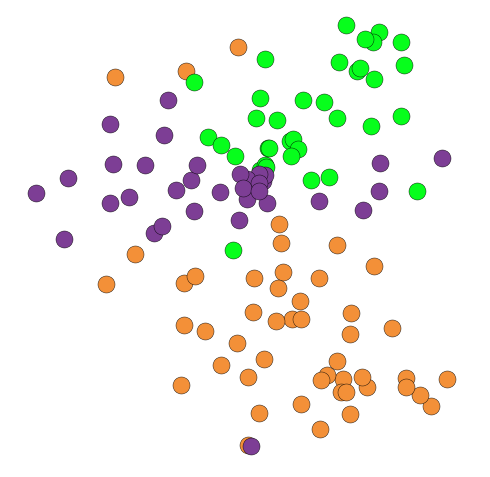
\includegraphics[width=0.23\linewidth , height=0.21\linewidth]{images/tsne_word2vec_raw_cities.png}}
\subcaptionbox{$r$GLV\label{sfig:glove_r_tsne}}{
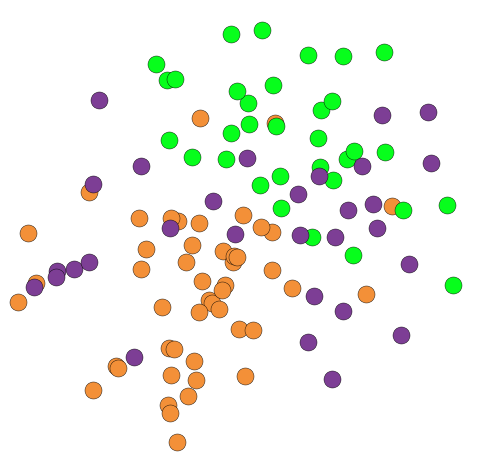
\includegraphics[width=0.23\linewidth , height=0.21\linewidth]{images/tsne_glove_raw_cities.png}}
\subcaptionbox{$a$W2V\label{sfig:word2vec_tsne}}{
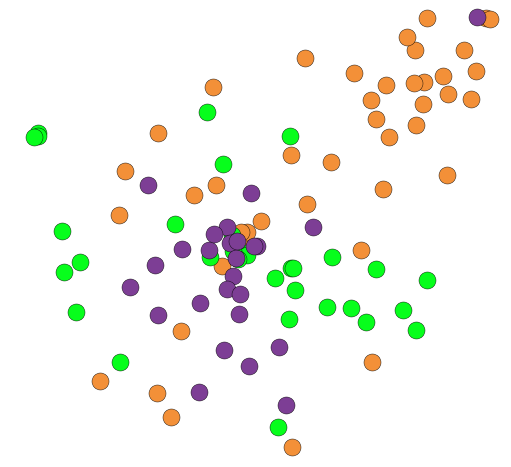
\includegraphics[width=0.23\linewidth , height=0.21\linewidth]{images/tsne_word2vec_cities.png}}
\subcaptionbox{$a$GLV\label{sfig:glove_tsne}}{
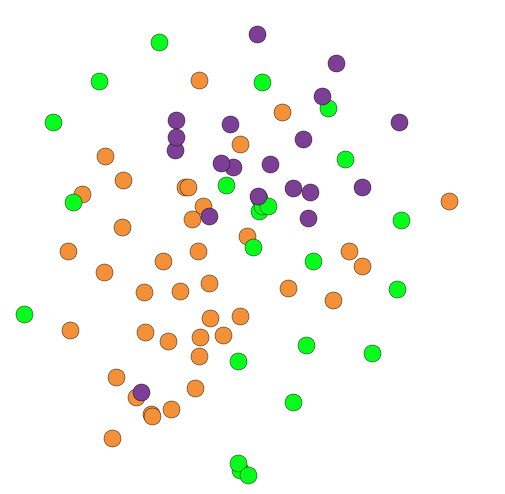
\includegraphics[width=0.23\linewidth , height=0.21\linewidth]{images/tsne_glove_cities.png}}
\subcaptionbox{DW$_{id}$\label{sfig:deepwalk_i_tsne}}{
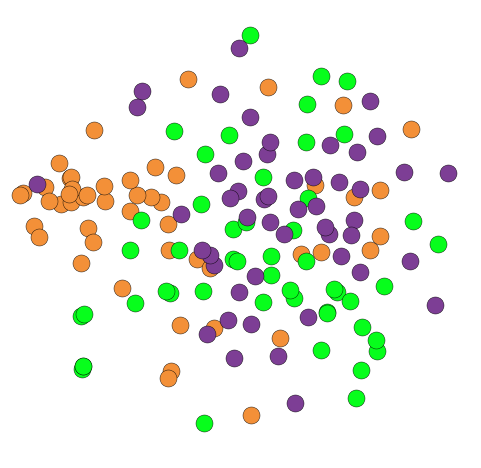
\includegraphics[width=0.23\linewidth , height=0.21\linewidth]{images/tsne_deepwalk_i_cities.png}}
\subcaptionbox{DW$_{log}$\label{sfig:deepwalk_l_tsne}}{
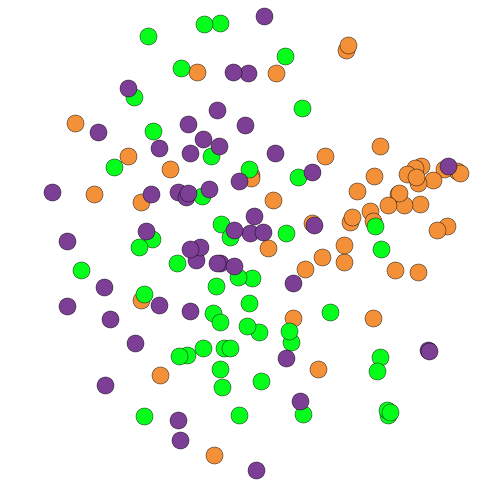
\includegraphics[width=0.23\linewidth , height=0.21\linewidth]{images/tsne_deepwalk_l_cities.png}}
\subcaptionbox{VRS\label{sfig:verse_tsne}}{
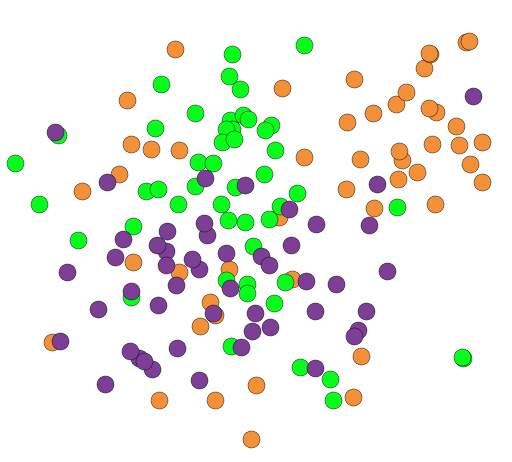
\includegraphics[width=0.23\linewidth , height=0.21\linewidth]{images/tsne_verse_cities.png}}
%\vspace*{-5pt}
\caption{t-SNE projections of the embeddings for U.S.\ (purple), British (orange), and German (green) cities. For the raw text models, multi-word entity names are represented as the mean of word vectors.}
\label{fig:clust}
%\vspace*{-8pt}
\end{figure}

%%%%%%%%%%%%%%%%%%%%%%%%%%%%%%%%%%%%%%%%%%%%%%%%%%%%%%%%%%%%
\subsubsection{Entity neighbourhoods} 
\begin{figure}[t]
\centering
\subcaptionbox{$r$W2V\label{sfig:obama_w2v_r}}{
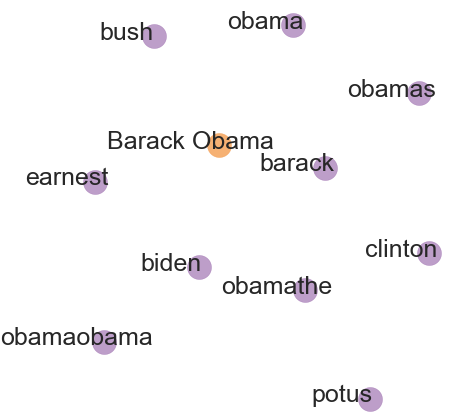
\includegraphics[width=0.30\linewidth , height=0.28\linewidth]{images/obama_w2v_r.png}}\hspace{12pt}%
\subcaptionbox{$a$W2V\label{sfig:obama_w2v}}{
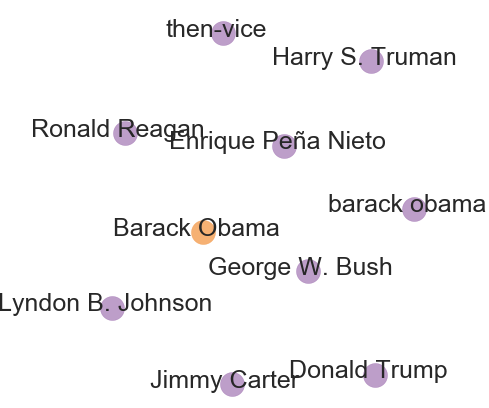
\includegraphics[width=0.30\linewidth , height=0.28\linewidth]{images/obama_w2v.png}}\hspace{12pt}%
\subcaptionbox{VRS\label{sfig:obama_verse}}{
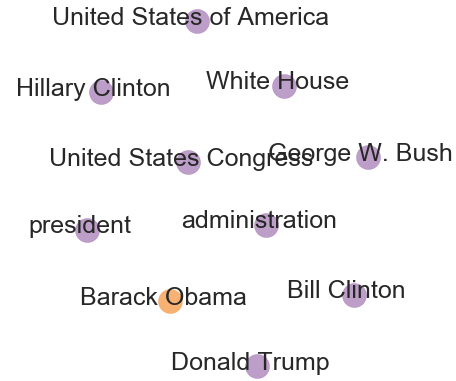
\includegraphics[width=0.30\linewidth , height=0.28\linewidth]{images/obama_verse.png}}
%\vspace*{-5pt}
\caption{t-SNE projections of the nearest neighbours of entity \emph{Barack Obama}.
 % for \emph{w2vec\_r} in  (\subref{sfig:obama_w2v_r}), \emph{w2vec} in  (\subref{sfig:obama_w2v}) and \emph{``Vrs"} in (\subref{sfig:obama_verse}).
}
\label{fig:obama}
%\vspace*{-15pt}
\end{figure}
To understand the neighbourhood relation and proximity of embeddings, we look at most similar word by cosine similarity on the example of the entity \emph{Barack Obama}. For the raw text models, we average the embeddings of the words \emph{barack} and \emph{obama}. A list of top five words is for all models are shown in Table~\ref{tbl:obama}. Entity-based models are more focused on related entities, whereas the the embeddings on raw text tend to focus more on surrounding terms. $r$W2V in particular retrieves mostly misspelled versions of the entity name, or it's separate components. Although these words are probably the most similar words in terms of semantic similarity (mostly synonyms that can substituted the entity name in a text), they do not give any further information about possible entity to entity relations. Once again, we observe that graph-based models on annotated text, VRS in particular, favours relatedness over similarity, as the top retrieved words are the related words that have some association to the entity in question. \\
The Figure~\ref{fig:clust} shows the neighbourhood of top ten closest words to \emph{Barack Obama} for $r$W2V, $a$W2V, and VRS. We observe a similar trend in the 2-dimensional t-SNE projections, where word2vec on raw text tends to primarily identifies synonymously used words on the raw corpus (i.e., variations of the entity name) and focuses on similarity. Word2vec on the annotated text, while retrieving more entities also favours similarity, as the nearest neighbours are either other presidents or entities that share similar roles. In contrast, VERSE identifies related entities with different roles, such as administrative locations or the presidential candidates and the president elect in the 2016 U.S.\ election.\\
Overall, for tasks that require word similarity word embedding methods tend to produce the best result, while the graph-based models have better performance when it comes to identifying relation or association between entities.
\begin{table}[t]
\caption{Four nearest neighbours of entity \emph{Barack Obama} with cosine similarity scores. Entity types include terms T, actors A, and locations L.}
\label{tbl:obama}
\setlength{\tabcolsep}{2pt} % Default value: 6pt
\renewcommand{\arraystretch}{1.0} % Default value: 1
\resizebox{\textwidth}{!}{%
\begin{tabular}{lllllllllllllll}
\toprule
\multicolumn{3}{c}{$r$W2V} & & \multicolumn{3}{c}{$r$GLV} & & \multicolumn{3}{c}{$a$W2V} & & \multicolumn{3}{c}{$a$GLV} \\
\cmidrule(lr){1-3}
\cmidrule(lr){5-7}
\cmidrule(lr){9-11}
\cmidrule(lr){13-15}
T & obama      & 0.90 &&  T & obama          & 0.99 && A & George W. Bush         & 0.76 && T & president      & 0.78 \\
T & barack     & 0.74 &&  T & barack         & 0.98 && A & Jimmy Carter           & 0.73 && T & administration & 0.76 \\
T & obamaobama & 0.68 &&  T & president      & 0.77 && T & barack obama           & 0.73 && A & George W. Bush & 0.72 \\
T & obamathe   & 0.60 &&  T & administration & 0.74 && A & Enrique Pe{\~n}a Nieto & 0.67 && T & mr.            & 0.68 \\
T & bush       & 0.55 &&  T & elect          & 0.66 && T & then-vice              & 0.67 && L & White House    & 0.67 \\
\bottomrule         
\end{tabular}%
}

\hspace*{21pt}
\resizebox{0.87\textwidth}{!}{
\begin{tabular}{lllllllllll}
\toprule
\multicolumn{3}{c}{DW$_{id}$} & & \multicolumn{3}{c}{DW$_{log}$} & & \multicolumn{3}{c}{VRS} \\
\cmidrule(lr){1-3}
\cmidrule(lr){5-7}
\cmidrule(lr){9-11} 
L & White House    & 0.88 && L & White House    & 0.88 && L & White House              & 0.87 \\
T & president      & 0.79 && T & president      & 0.82 && T & president                & 0.79 \\ 
T & presidency     & 0.76 && A & George W. Bush & 0.78 && L & United States of America & 0.76 \\
T & administration & 0.75 && T & administration & 0.78 && A & Donald Trump             & 0.75 \\
A & George W. Bush & 0.74 && T & presidency     & 0.78 && A & Hillary Clinton          & 0.74 \\
\bottomrule
\end{tabular}%
}
\end{table}
\subsection{Analysis of faceted embeddings}\label{subsec:exp_faceted}
To analysis the separate components of faceted embeddings and investigate the semantics behind them, we consider visualizing the clustering task and analysing the neighbourhood for entities. In both cases, we look at the full embeddings with all the components concatenated and also analyse each component separately to understand how the different types of entities surrounding a word can contribute to its semantics and affect it's relations to other entities.
%%%%%%%%%%%%%%%%%%%%%%%%%%%%%%%%%%%%%%%%
\subsubsection{Entity clustering} 
One way to understand which component is significant for representation of entities is to asses which component clusters the similar entities in the embedding. To achieve this, we project the full and partial embeddings of each component for the Cities dataset, which contains location entities, in a 2-dimensional space using t-SNE. The projection for  $f$DW$_{log}$ and $f$W2V are shown in Figure~\ref{fig:clust_fword2vec} and  Figure~\ref{fig:clust_fdeepwalk}, respectively. The subscript shows the embedding component that is used, e.g., $f$W2V$_{ACT}$ corresponds to facetted word2vec, using only the actor component and $f$W2V indicates the full embedding. Since the performance of $f$DW$_{id}$ and  $f$DW$_{log}$ are similar, we only illustrate the result for $f$DW$_{log}$. For both faceted models, it is not obvious what each component represents. None of the components of  $f$DW$_{log}$ form any meaningful cluster, however, the distinction between the three countries is somewhat visible for the location component. The faceted word2vec clearly indicates that dates surrounding a city name are not a good factor for their distinction as all the names are mapped to the same point. Two separate clusters are visible for the location component of $f$W2V, but they are not separated by the county of origin as both clusters are mixture of all three countries. In general, for the faceted models the visualization of the full embedding is closely related to term component, which is the dominate part in these models. 
\begin{figure}[t]
\centering
\subcaptionbox{$f$W2V$_{ACT}$\label{sfig:fword2vec_act_tsne}}{
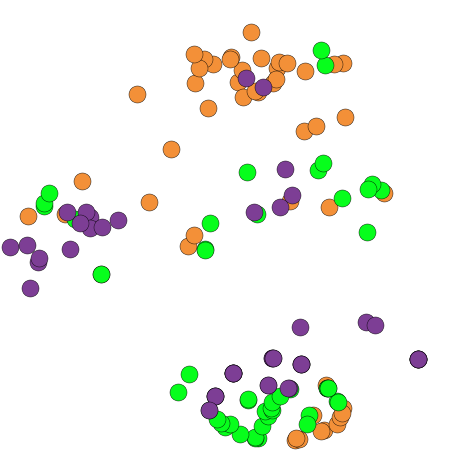
\includegraphics[width=0.23\linewidth , height=0.21\linewidth]{images/fword2vec_act_tsne.png}}
\subcaptionbox{$f$W2V$_{LOC}$\label{fig:fword2vec_loc_tsne}}{
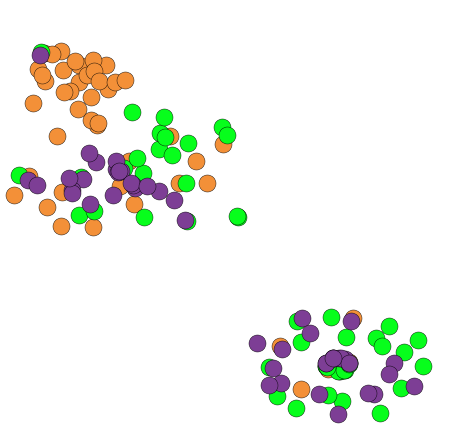
\includegraphics[width=0.23\linewidth , height=0.21\linewidth]{images/fword2vec_loc_tsne.png}}
\subcaptionbox{$f$W2V$_{ORG}$\label{sfig:fword2vec_org_tsne}}{
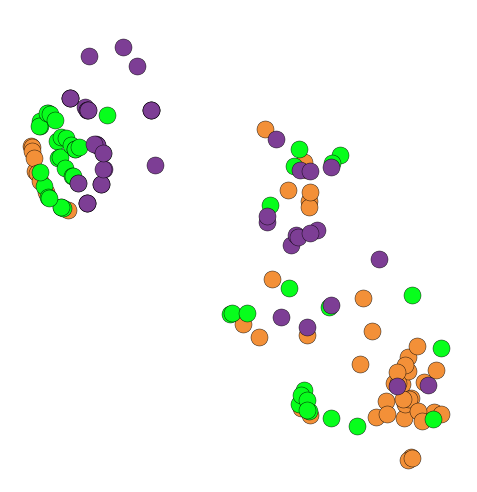
\includegraphics[width=0.23\linewidth , height=0.21\linewidth]{images/fword2vec_org_tsne.png}}
\subcaptionbox{$f$W2V$_{DAT}$\label{sfig:fword2vec_dat_tsne}}{
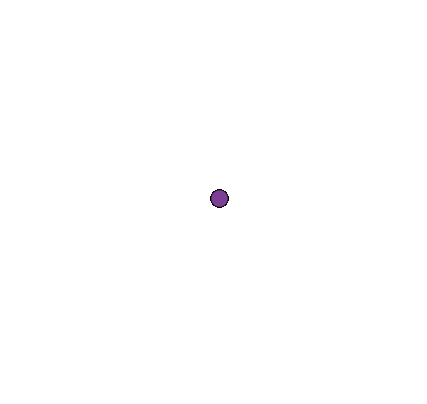
\includegraphics[width=0.23\linewidth , height=0.21\linewidth]{images/fword2vec_dat_tsne.png}}
\subcaptionbox{$f$W2V$_{TER}$\label{sfig:fword2vec_ter_tsne}}{
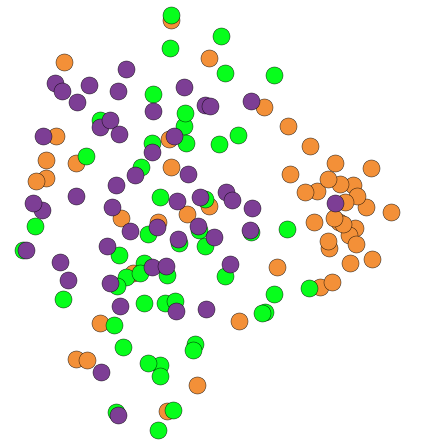
\includegraphics[width=0.23\linewidth , height=0.21\linewidth]{images/fword2vec_ter_tsne.png}}
\subcaptionbox{$f$W2V\label{sfig:fword2vec_tsne}}{
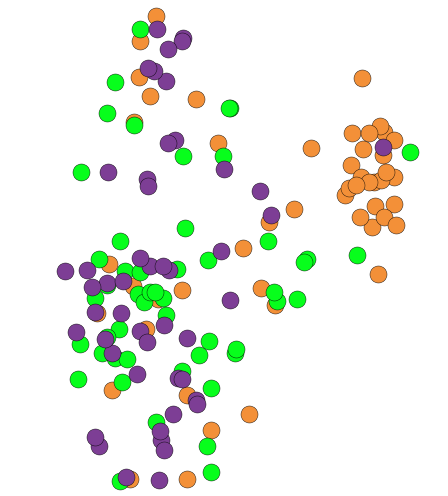
\includegraphics[width=0.23\linewidth , height=0.21\linewidth]{images/fword2vec_tsne.png}}
\caption{t-SNE projections of the embeddings for U.S.\ (purple), British (orange), and German (green) cities, for facetted word2vec using different components. }
\label{fig:clust_fword2vec}
\end{figure}

\begin{figure}[t]
\centering
\subcaptionbox{$f$DW$_{ACT}$\label{sfig:fdeepwalk_act_tsne}}{
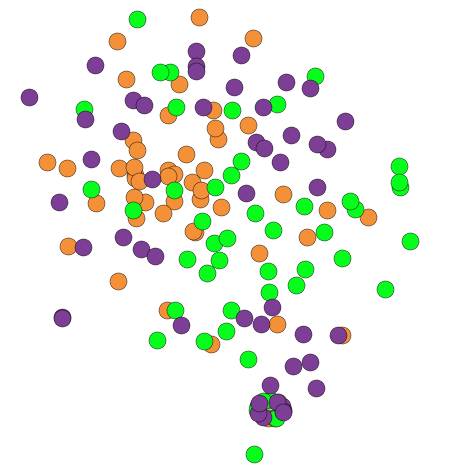
\includegraphics[width=0.23\linewidth , height=0.21\linewidth]{images/fdeepwalk_act_tsne.png}}
\subcaptionbox{$f$DW$_{LOC}$\label{fig:fdeepwalk_loc_tsne}}{
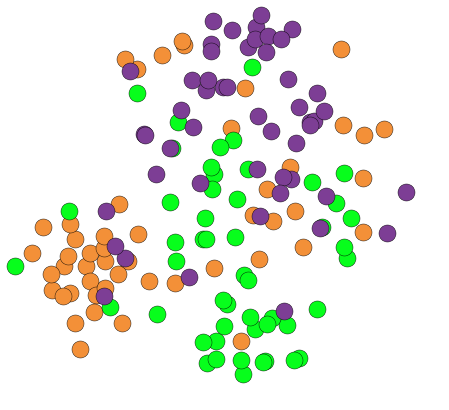
\includegraphics[width=0.23\linewidth , height=0.21\linewidth]{images/fdeepwalk_loc_tsne.png}}
\subcaptionbox{$f$DW$_{ORG}$\label{sfig:fdeepwalk_org_tsne}}{
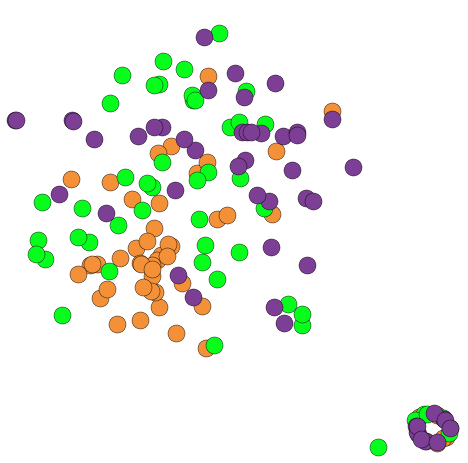
\includegraphics[width=0.23\linewidth , height=0.21\linewidth]{images/fdeepwalk_org_tsne.png}}
\subcaptionbox{$f$DW$_{DAT}$\label{sfig:fdeepwalk_dat_tsne}}{
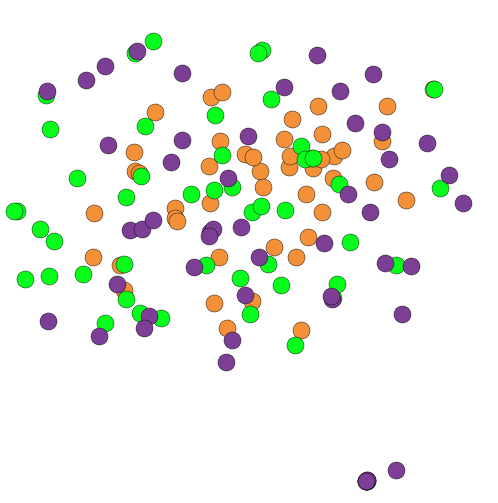
\includegraphics[width=0.23\linewidth , height=0.21\linewidth]{images/fdeepwalk_dat_tsne.png}}
\subcaptionbox{$f$DW$_{TER}$\label{sfig:fdeepwalk_ter_tsne}}{
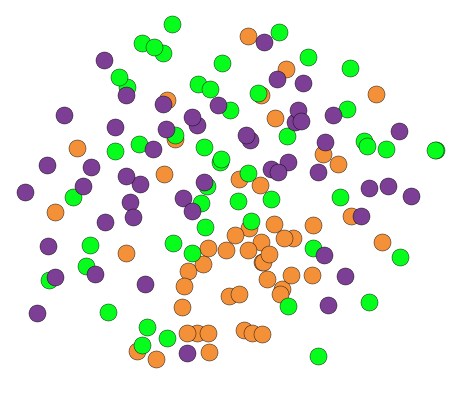
\includegraphics[width=0.23\linewidth , height=0.21\linewidth]{images/fdeepwalk_ter_tsne.png}}
\subcaptionbox{$f$DW\label{sfig:fdeepwalk_tsne}}{
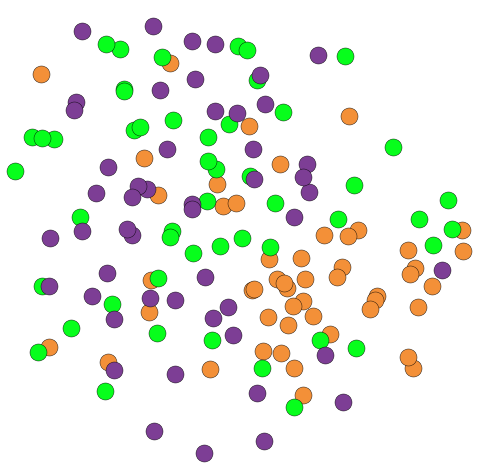
\includegraphics[width=0.23\linewidth , height=0.21\linewidth]{images/fdeepwalk_tsne.png}}
\caption{t-SNE projections of the embeddings for U.S.\ (purple), British (orange), and German (green) cities, for facetted deepwalk with logarithmic normalization using different components. }
\label{fig:clust_fdeepwalk}
\end{figure}

%%%%%%%%%%%%%%%%%%%%%%%%%%%%%%%%%%%%%%%%%%%%%%%%%%%%%%%%%%%%
\subsubsection{Entity neighbourhoods} 
To analyse the proximity of embeddings based on different components, we investigate the most similar words by cosine similarity to the example actor entity \emph{Barach Obama}. A list of top five words for the faceted models with full embedding and $r$W2V and $r$GLV is shown in Table~\ref{tbl:obama_faceted}. Same as the entity embeddings, the faceted models are more focused on entity relations, whereas the word embeddings on raw text retrieve synonymous terms. Although the $f$DW$_{id}$ tends to contain some terms in the top result, with the log normalization the result become close to $f$W2V,which mostly contains former presidents, the presidential candidate for 2016 election and other democrat politicians. In Table~\ref{tbl:obama_faceted_p} we look at the top five results based on separate components for $f$W2V and $f$DW$_{log}$, where the subscript indicates the component that is used to find the nearest neighbours. $f$DW$_{id}$ produces similar results and, thus, is not demonstrated. 
\begin{table}[t]
\caption{Four nearest neighbours of entity \emph{Barack Obama} with cosine similarity scores for faceted models and embeddings on raw text. Entity types include terms T and actors A.}
\label{tbl:obama_faceted}
\setlength{\tabcolsep}{1.5pt} % Default value: 6pt
\renewcommand{\arraystretch}{1.0} % Default value: 1
\resizebox{\textwidth}{!}{%
\begin{tabular}{lllllllllllllllllll}
\toprule
\multicolumn{3}{c}{$r$W2V} & & \multicolumn{3}{c}{$r$GLV} & & \multicolumn{3}{c}{$f$W2V} & & \multicolumn{3}{c}{$f$DW$_{id}$} & & \multicolumn{3}{c}{$f$DW$_{log}$}\\
\cmidrule(lr){1-3}
\cmidrule(lr){5-7}
\cmidrule(lr){9-11}
\cmidrule(lr){13-15}
\cmidrule(lr){17-19}
T & obama      & 0.90 &&  T & obama     & 0.99 && A & Donald Trump & 0.92    && A & Donald Trump & 0.84&& A& Hillary Clinton & 0.85 \\
T & barack     & 0.74 &&  T & barack         & 0.98 && A & Hillary Clinton & 0.91 && A & Hillary Clinton & 0.84 && A & Donald Trump & 0.85\\
T & obamaobama & 0.68 &&  T & president      & 0.77 && A & Bill Clinton & 0.89 && T & nation & 0.83 && A & Bill Clinton & 0.83\\
T & obamathe   & 0.60 &&  T & administration & 0.74 && A & Bernie Sanders & 0.87 && T & force & 0.83 && A & Josh Earnest & 0.82 \\
T & bush       & 0.55 &&  T & elect          & 0.66 && A & George W. Bush & 0.87 && T & freedom & 0.82 && T & administration & 0.82\\
\bottomrule         
\end{tabular}%
}
\end{table}


\begin{table}[t]
\caption{Four nearest neighbours of entity \emph{Barack Obama} with cosine similarity scores .for separate components of $f$W2V and $f$DW$_{log}$. Entity types include terms T, actors A , and locations L, organisations O, dates D.}
\label{tbl:obama_faceted_p}
\setlength{\tabcolsep}{1.5pt} % Default value: 6pt
\renewcommand{\arraystretch}{1.0} % Default value: 1
\resizebox{\textwidth}{!}{%
\begin{tabular}{lllllllllllllllllll}
\toprule
\multicolumn{3}{c}{$f$W2V$_{TER}$} & & \multicolumn{3}{c}{$f$W2V$_{ACT}$} & & \multicolumn{3}{c}{$f$W2V$_{LOC}$} & & \multicolumn{3}{c}{$f$W2V$_{ORG}$} & & \multicolumn{3}{c}{$f$W2V$_{DAT}$}\\
\cmidrule(lr){1-3}
\cmidrule(lr){5-7}
\cmidrule(lr){9-11}
\cmidrule(lr){13-15}
\cmidrule(lr){17-19}
L &White House & 0.97&& L & White House & 0.98 && T & 0324 & 0.77  && A & White House & 0.97&& D & 2016-01-26 & 0.64 \\
T & democratic & 0.96&&  A & Donald Trump & 0.92&& L & St. John's Episcopal Church & 0.76 && A & Donald Trump & 0.93 && D & 2008-06-08 & 0.57\\
T & presidential & 0.95 &&  L & Washington, D.C. & 0.92&& D & 2011-07-09 & 0.73 && O & U.S House of Representatives & 0.93 && D & 2005 & 0.56\\
A & George W. Bush & 0.94 && A & Ben Rhodes & 0.91&& L & South Sudan & 0.72 && O & U.S Congress & 0.93 && D & 1865-05 & 0.56 \\
T & republican & 0.94&&  A & Hillary Clinton & 0.91 && L & Palazzo Grassi & 0.71&& A & fHillary Clinton & 0.93&& D & 1970 & 0.55\\
\bottomrule         
\end{tabular}%
}

\resizebox{\textwidth}{!}{
\begin{tabular}{lllllllllllllllllll}
\toprule
\multicolumn{3}{c}{$f$DW$_{TER}$} & & \multicolumn{3}{c}{$f$DW$_{ACT}$} & & \multicolumn{3}{c}{$f$DW$_{LOC}$} & & \multicolumn{3}{c}{$f$DW$_{ORG}$} & & \multicolumn{3}{c}{$f$DW$_{DAT}$}\\
\cmidrule(lr){1-3}
\cmidrule(lr){5-7}
\cmidrule(lr){9-11}
\cmidrule(lr){13-15}
\cmidrule(lr){17-19}
L &Philadelphia & 0.94&& A & Daniel M. Ashe & 0.92 && T & decades & 0.97  && A & Bill Clinton & 0.97&& T & not & 0.99 \\
L & Pennsylvania & 0.94&&  A & Hefty Stuart & 0.90&& T & reported & 0.97 && L & New York City & 0.96 && L & Alabama & 0.99\\
D & 2016-07 & 0.92 &&  A & Elena Bromund & 0.90&& T & statement & 0.96 && T & according & 0.95 && T & party & 0.99\\
L & New York City & 0.92 && A & Brendan O'Connor & 0.90&& T & rally & 0.96 && A & Donald Trump & 0.95 && T & timeline & 0.98 \\
O & United States Congress & 0.92 &&  A & Glenn Hutchins & 0.90 && T & according & 0.96&& L & Benghazi & 0.95&& D & kept & 0.98\\
\bottomrule         
\end{tabular}%
}
\end{table}
%-----removed parts 
%
%\begin{figure}
%\centering
%\subcaptionbox{\label{sfig:full_wordsim}}{
%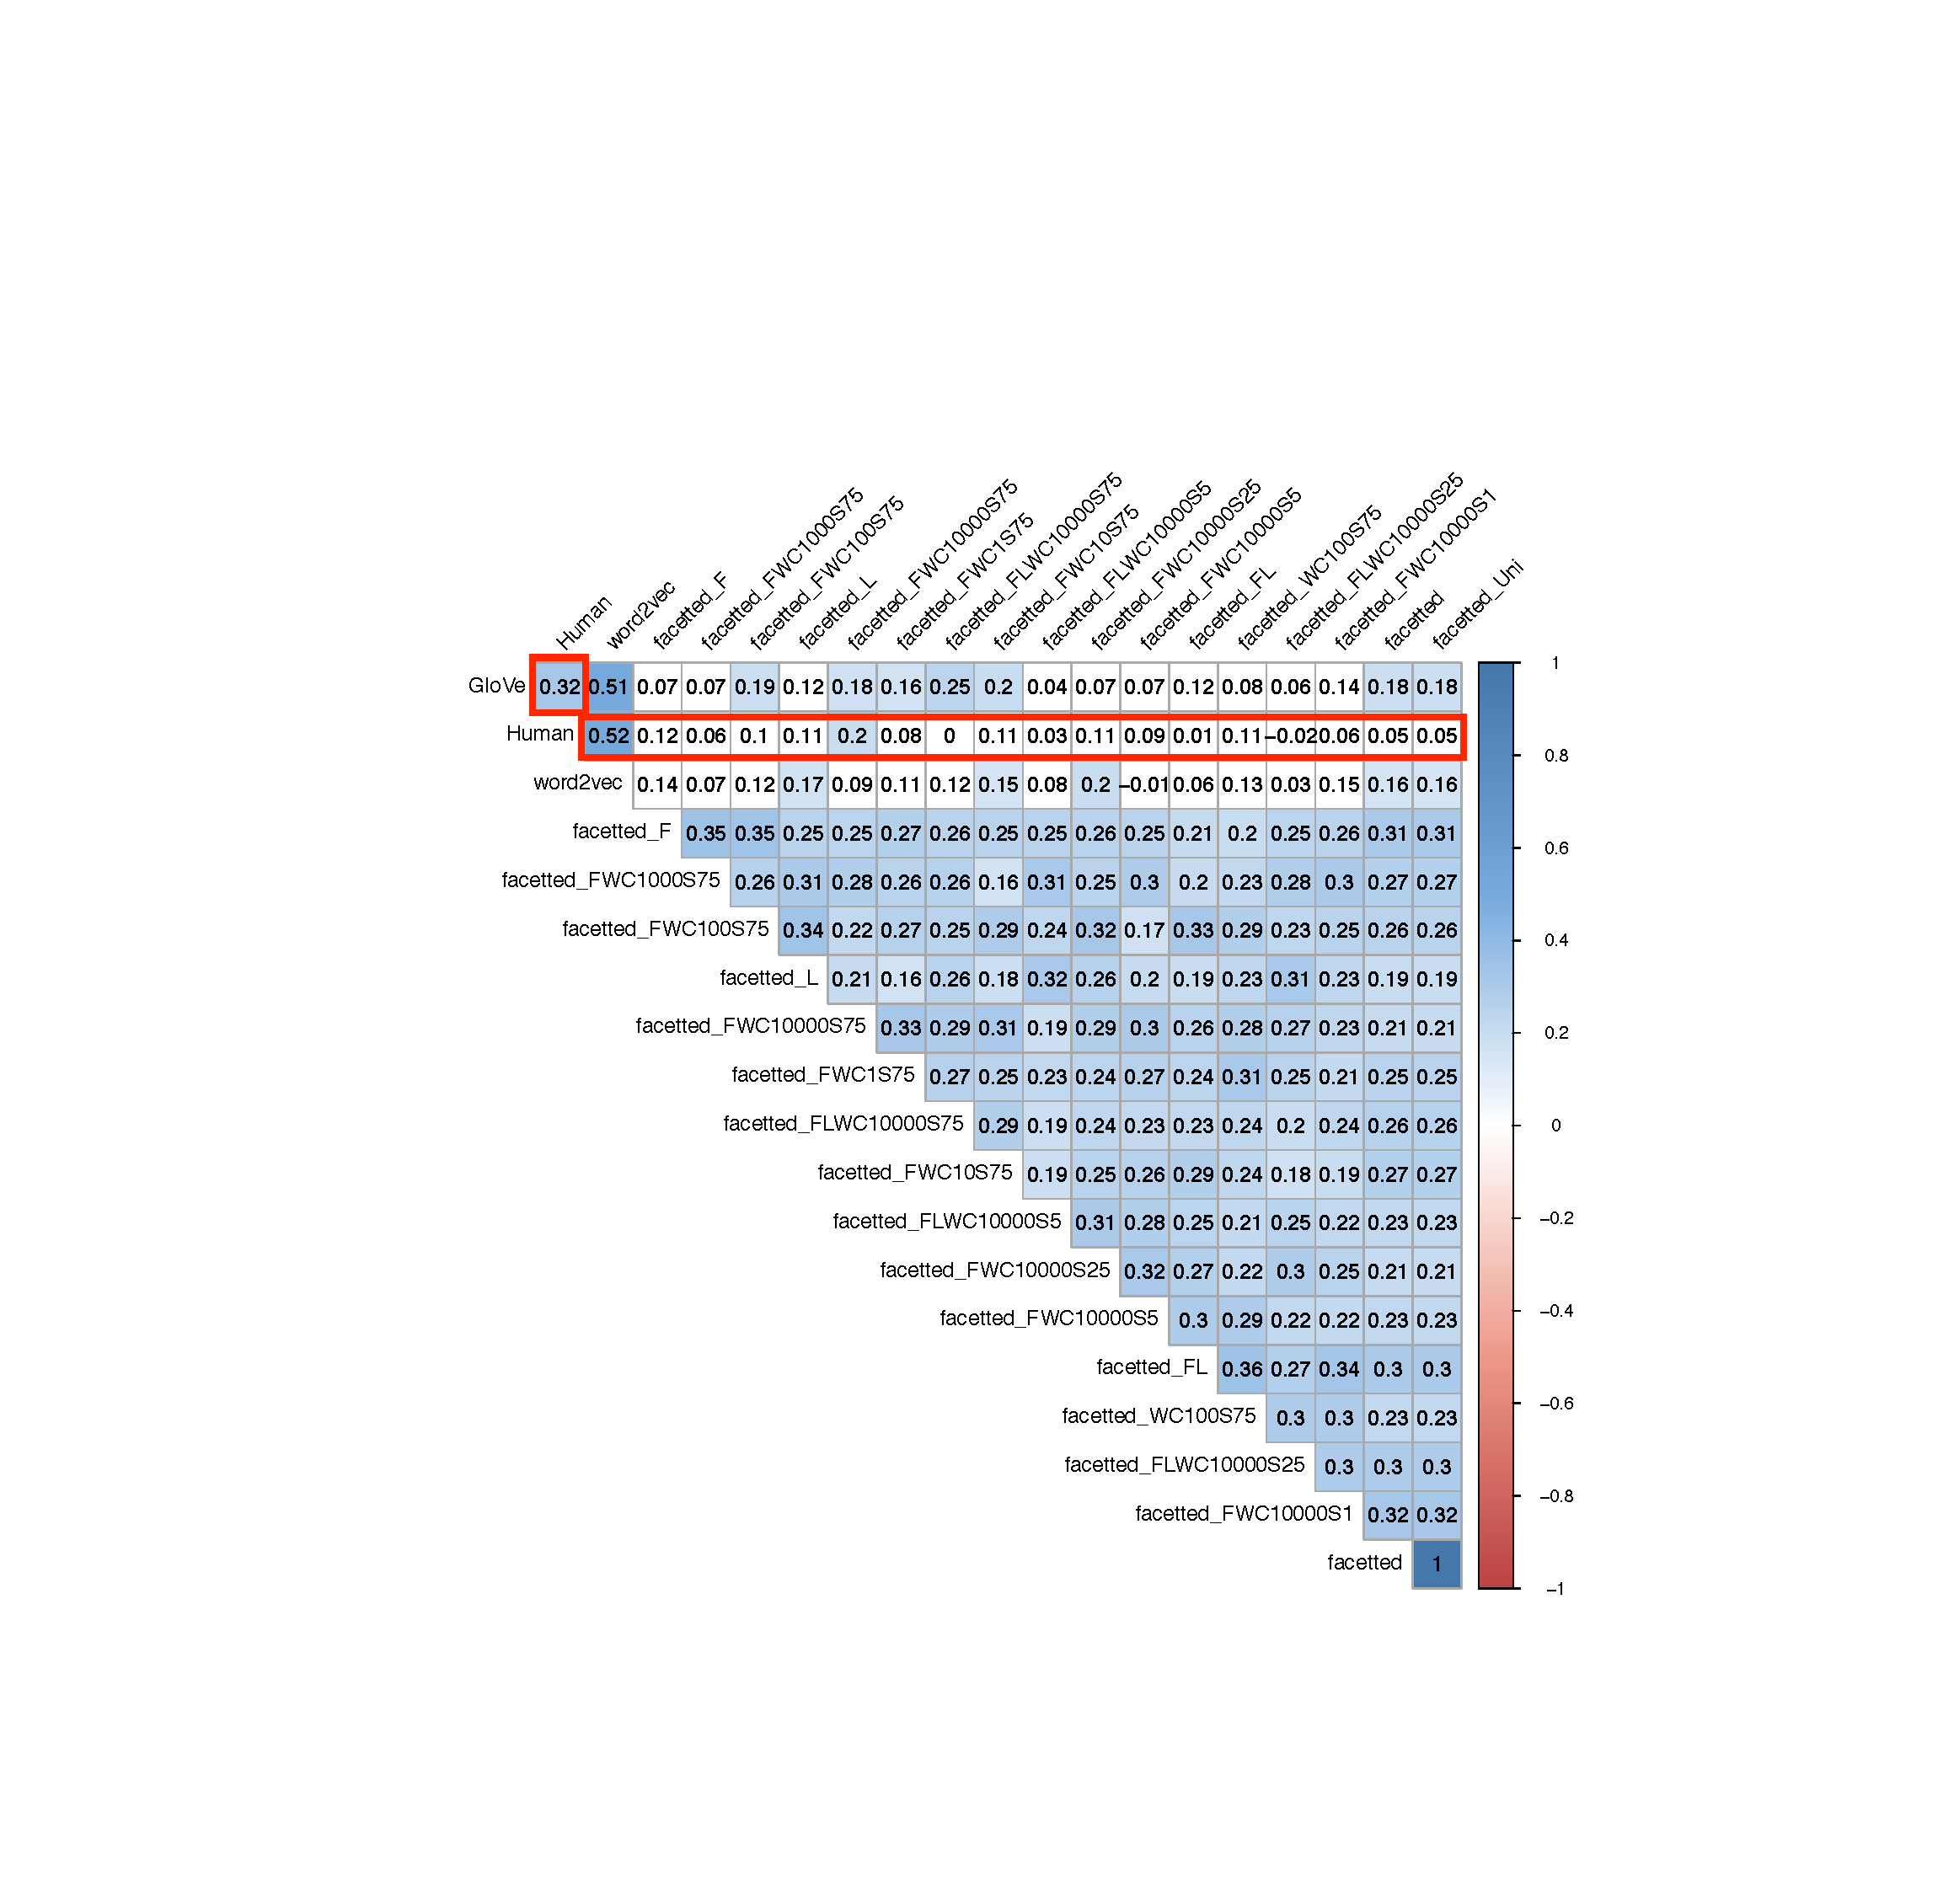
\includegraphics[width=0.75\linewidth , height=0.65\linewidth]{images/Corr_plot_full_sim.pdf}}
%\subcaptionbox{\label{sfig:part_wordsim}}{
%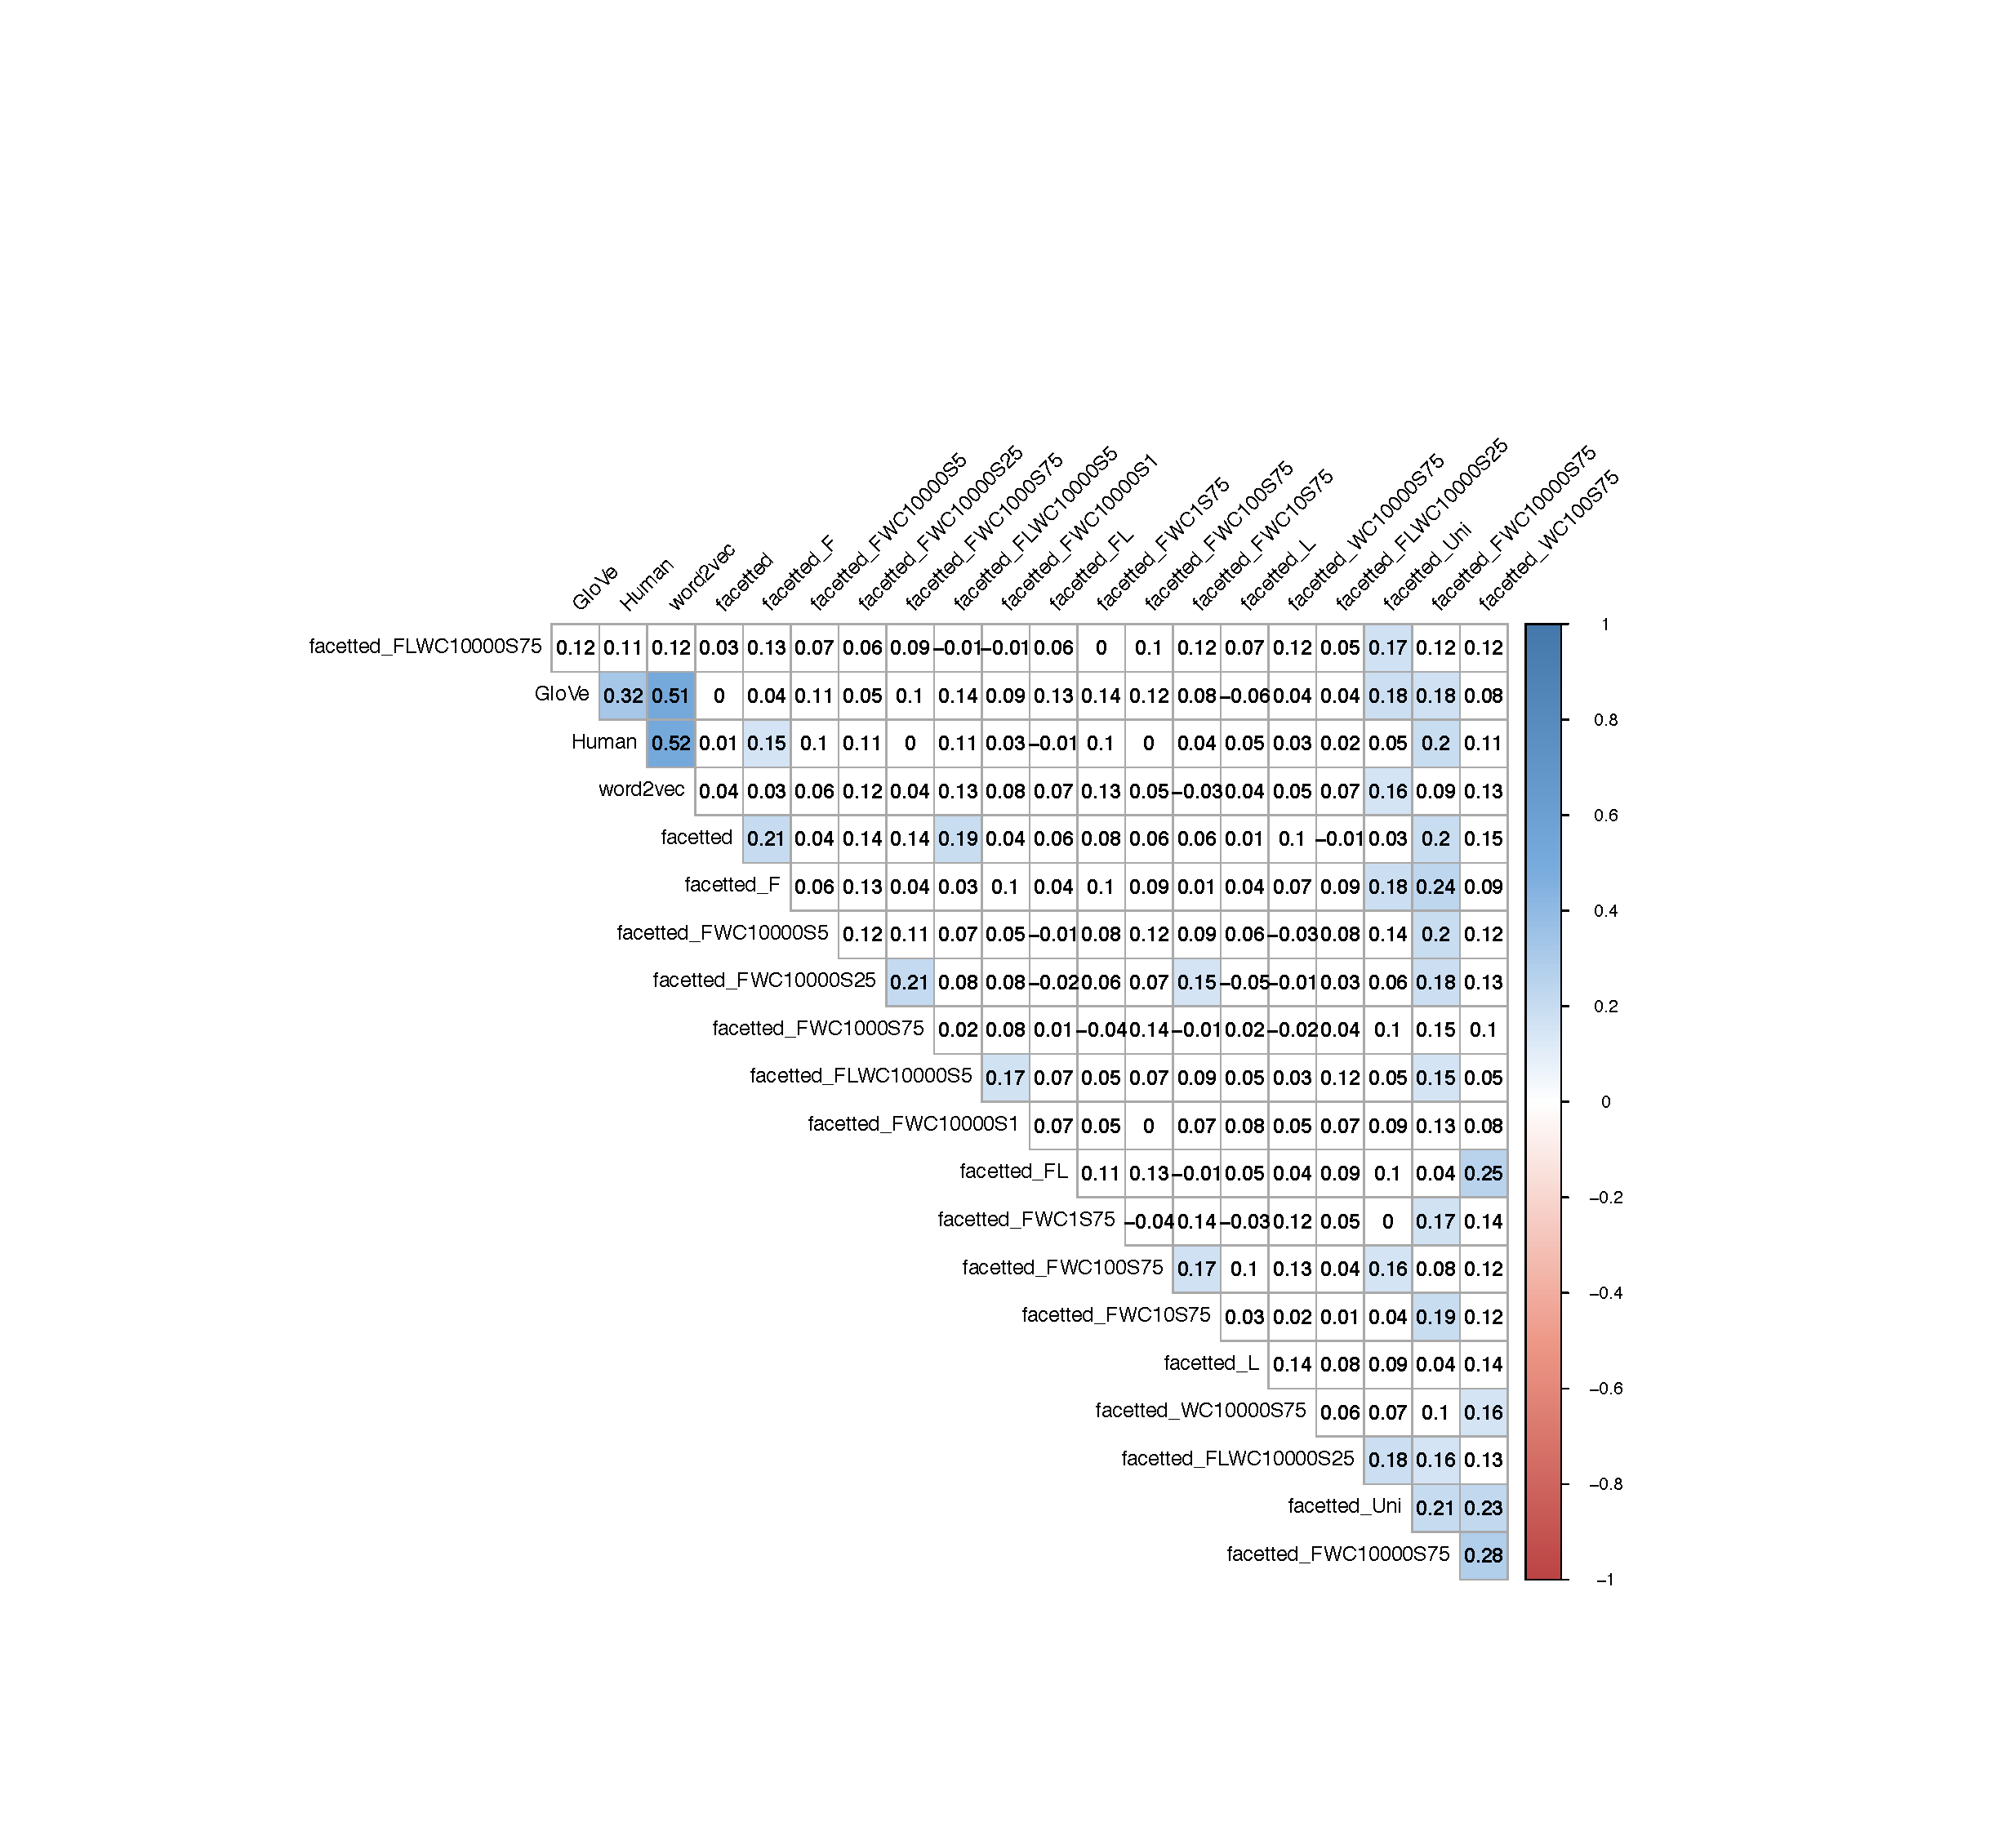
\includegraphics[width=0.80\linewidth , height=0.65\linewidth]{images/wordsim_partial.pdf}}
%
%\caption{Correlation plot of the relatedness scores on wordsim353 using the~\subref{sfig:full_wordsim} full vectors and ~\subref{sfig:part_wordsim} using type-specific vectors. Red highlights show the correlation with the human annotations.}
%\label{fig:wordsim_cor}
%\end{figure}
%
%
%%\begin{figure}
%\centering
%\subcaptionbox{\label{sfig:word2vec_tsne}}{
%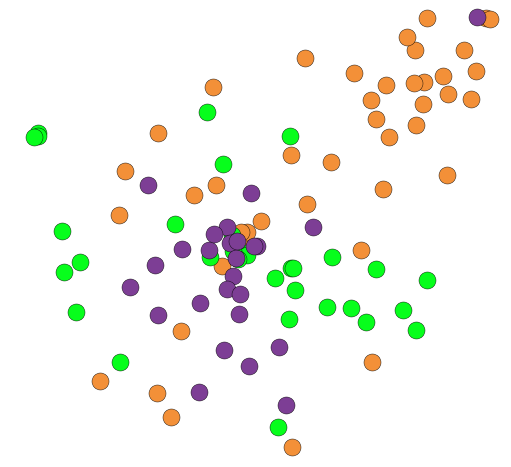
\includegraphics[width=0.48\linewidth , height=0.5\linewidth]{images/tsne_word2vec_cities.png}}
%\subcaptionbox{\label{sfig:glove_tsne}}{
%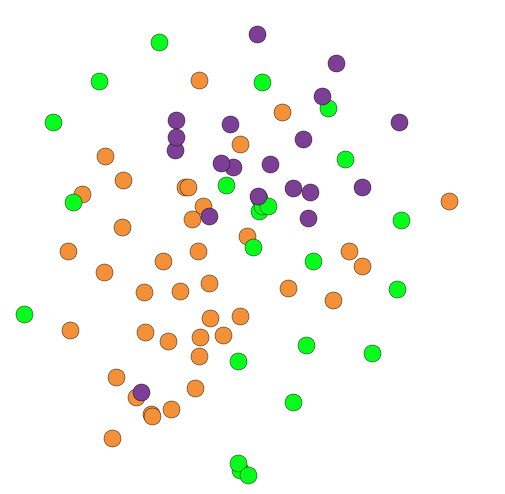
\includegraphics[width=0.48\linewidth , height=0.5\linewidth]{images/tsne_glove_cities.png}}
%\subcaptionbox{\label{sfig:complex_tsne}}{
%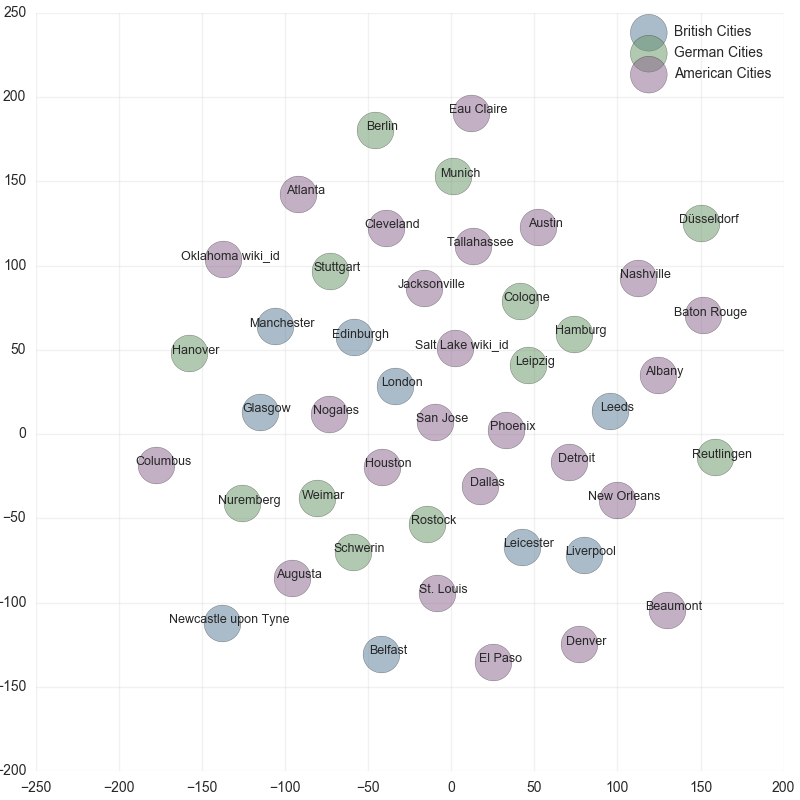
\includegraphics[width=0.5\linewidth , height=0.5\linewidth]{images/tsne_complex_cities.png}}
%
%\caption{t-SNE projections of the embeddings:\subref{sfig:word2vec_tsne} German, British and American cities using Word2Vec \subref{sfig:glove_tsne} GloVe and \subref{sfig:complex_tsne} facetted\_FWC10000S75.}
%\label{fig:clust}
%\end{figure}
%
%
%\begin{table}[h]
%  \centering
%  {%
%    \raisebox{1.5cm}{%
%      \begin{tabular}{lSS}
%        \toprule
%        {Algorithm }                     & {Accuracy}   \\
%        \midrule
%        Facetted\_FWC10000S75   &0        \\
%        GloVe    & 0.008     \\
%        word2vec   & 0.015       \\
%        \bottomrule
%      \end{tabular}
%    }
%  }
%  \caption{The accuracy results on Mikolove's test set with $9,968$ word pairs.}
%  \label{table:analogy}
%\end{table}
%
%
%\begin{figure}[hb]
%\centering
%\subcaptionbox{\label{sfig:scaling_f}}{
%\resizebox{0.45\textwidth}{0.30\textwidth}{      
%
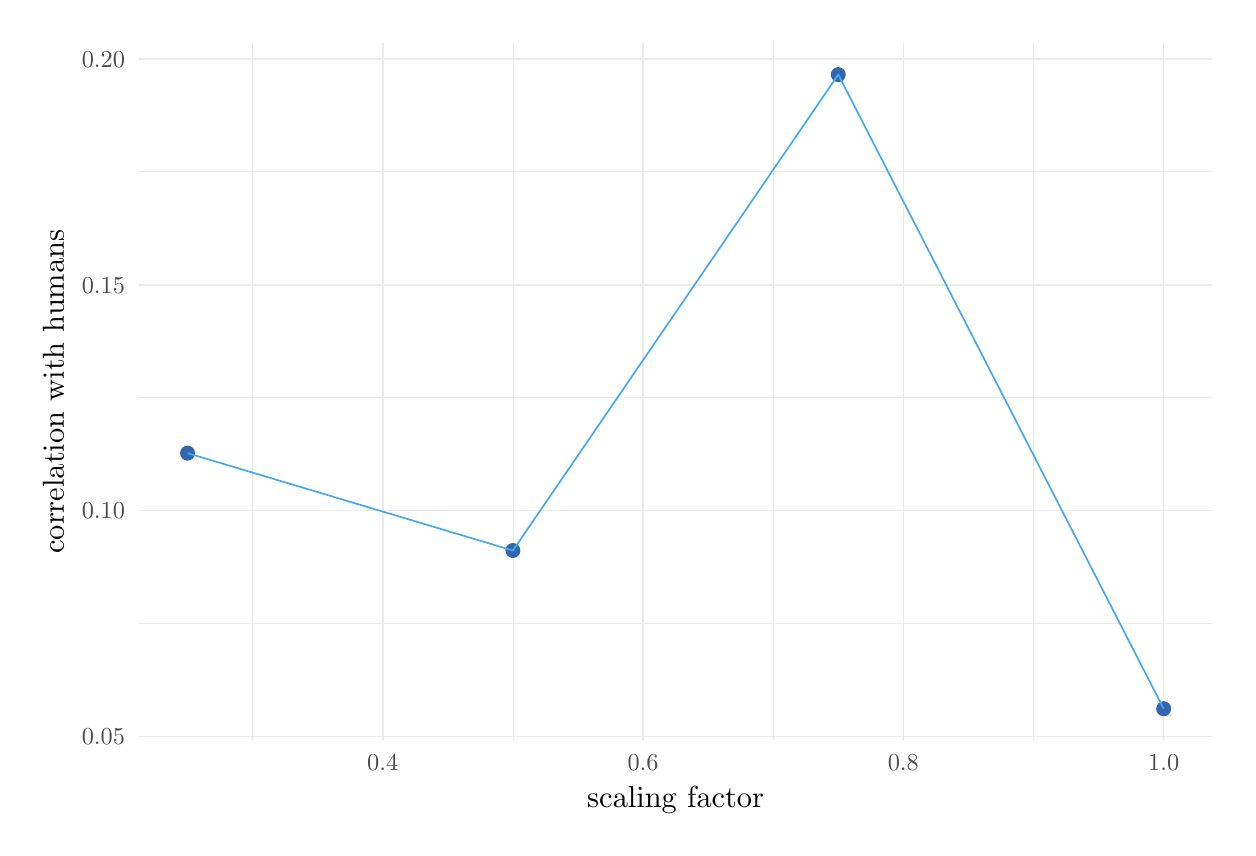
\begin{tikzpicture}[x=1pt,y=1pt]
\definecolor{fillColor}{RGB}{255,255,255}
\path[use as bounding box,fill=fillColor,fill opacity=0.00] (0,0) rectangle (433.62,289.08);
\begin{scope}
\path[clip] ( 40.14, 31.53) rectangle (428.12,283.58);
\definecolor{drawColor}{gray}{0.92}

\path[draw=drawColor,line width= 0.3pt,line join=round] ( 40.14, 73.78) --
	(428.12, 73.78);

\path[draw=drawColor,line width= 0.3pt,line join=round] ( 40.14,155.37) --
	(428.12,155.37);

\path[draw=drawColor,line width= 0.3pt,line join=round] ( 40.14,236.97) --
	(428.12,236.97);

\path[draw=drawColor,line width= 0.3pt,line join=round] ( 81.29, 31.53) --
	( 81.29,283.58);

\path[draw=drawColor,line width= 0.3pt,line join=round] (175.34, 31.53) --
	(175.34,283.58);

\path[draw=drawColor,line width= 0.3pt,line join=round] (269.40, 31.53) --
	(269.40,283.58);

\path[draw=drawColor,line width= 0.3pt,line join=round] (363.46, 31.53) --
	(363.46,283.58);

\path[draw=drawColor,line width= 0.6pt,line join=round] ( 40.14, 32.98) --
	(428.12, 32.98);

\path[draw=drawColor,line width= 0.6pt,line join=round] ( 40.14,114.58) --
	(428.12,114.58);

\path[draw=drawColor,line width= 0.6pt,line join=round] ( 40.14,196.17) --
	(428.12,196.17);

\path[draw=drawColor,line width= 0.6pt,line join=round] ( 40.14,277.76) --
	(428.12,277.76);

\path[draw=drawColor,line width= 0.6pt,line join=round] (128.32, 31.53) --
	(128.32,283.58);

\path[draw=drawColor,line width= 0.6pt,line join=round] (222.37, 31.53) --
	(222.37,283.58);

\path[draw=drawColor,line width= 0.6pt,line join=round] (316.43, 31.53) --
	(316.43,283.58);

\path[draw=drawColor,line width= 0.6pt,line join=round] (410.48, 31.53) --
	(410.48,283.58);
\definecolor{drawColor}{RGB}{50,103,173}
\definecolor{fillColor}{RGB}{50,103,173}

\path[draw=drawColor,line width= 0.4pt,line join=round,line cap=round,fill=fillColor] ( 57.77,135.33) circle (  2.50);

\path[draw=drawColor,line width= 0.4pt,line join=round,line cap=round,fill=fillColor] (175.34,100.15) circle (  2.50);

\path[draw=drawColor,line width= 0.4pt,line join=round,line cap=round,fill=fillColor] (292.91,272.12) circle (  2.50);

\path[draw=drawColor,line width= 0.4pt,line join=round,line cap=round,fill=fillColor] (410.48, 42.99) circle (  2.50);
\definecolor{drawColor}{RGB}{66,167,244}

\path[draw=drawColor,line width= 0.6pt,line join=round] ( 57.77,135.33) --
	(175.34,100.15) --
	(292.91,272.12) --
	(410.48, 42.99);
\end{scope}
\begin{scope}
\path[clip] (  0.00,  0.00) rectangle (433.62,289.08);
\definecolor{drawColor}{gray}{0.30}

\node[text=drawColor,anchor=base east,inner sep=0pt, outer sep=0pt, scale=  0.88] at ( 35.19, 29.95) {0.05};

\node[text=drawColor,anchor=base east,inner sep=0pt, outer sep=0pt, scale=  0.88] at ( 35.19,111.55) {0.10};

\node[text=drawColor,anchor=base east,inner sep=0pt, outer sep=0pt, scale=  0.88] at ( 35.19,193.14) {0.15};

\node[text=drawColor,anchor=base east,inner sep=0pt, outer sep=0pt, scale=  0.88] at ( 35.19,274.73) {0.20};
\end{scope}
\begin{scope}
\path[clip] (  0.00,  0.00) rectangle (433.62,289.08);
\definecolor{drawColor}{gray}{0.30}

\node[text=drawColor,anchor=base,inner sep=0pt, outer sep=0pt, scale=  0.88] at (128.32, 20.52) {0.4};

\node[text=drawColor,anchor=base,inner sep=0pt, outer sep=0pt, scale=  0.88] at (222.37, 20.52) {0.6};

\node[text=drawColor,anchor=base,inner sep=0pt, outer sep=0pt, scale=  0.88] at (316.43, 20.52) {0.8};

\node[text=drawColor,anchor=base,inner sep=0pt, outer sep=0pt, scale=  0.88] at (410.48, 20.52) {1.0};
\end{scope}
\begin{scope}
\path[clip] (  0.00,  0.00) rectangle (433.62,289.08);
\definecolor{drawColor}{RGB}{0,0,0}

\node[text=drawColor,anchor=base,inner sep=0pt, outer sep=0pt, scale=  1.10] at (234.13,  7.44) {scaling factor};
\end{scope}
\begin{scope}
\path[clip] (  0.00,  0.00) rectangle (433.62,289.08);
\definecolor{drawColor}{RGB}{0,0,0}

\node[text=drawColor,rotate= 90.00,anchor=base,inner sep=0pt, outer sep=0pt, scale=  1.10] at ( 13.08,157.56) {correlation with humans};
\end{scope}
\end{tikzpicture}


%}}
%\subcaptionbox{\label{sfig:weight_cap}}{\resizebox{0.45\textwidth}{0.30\textwidth}{      
%
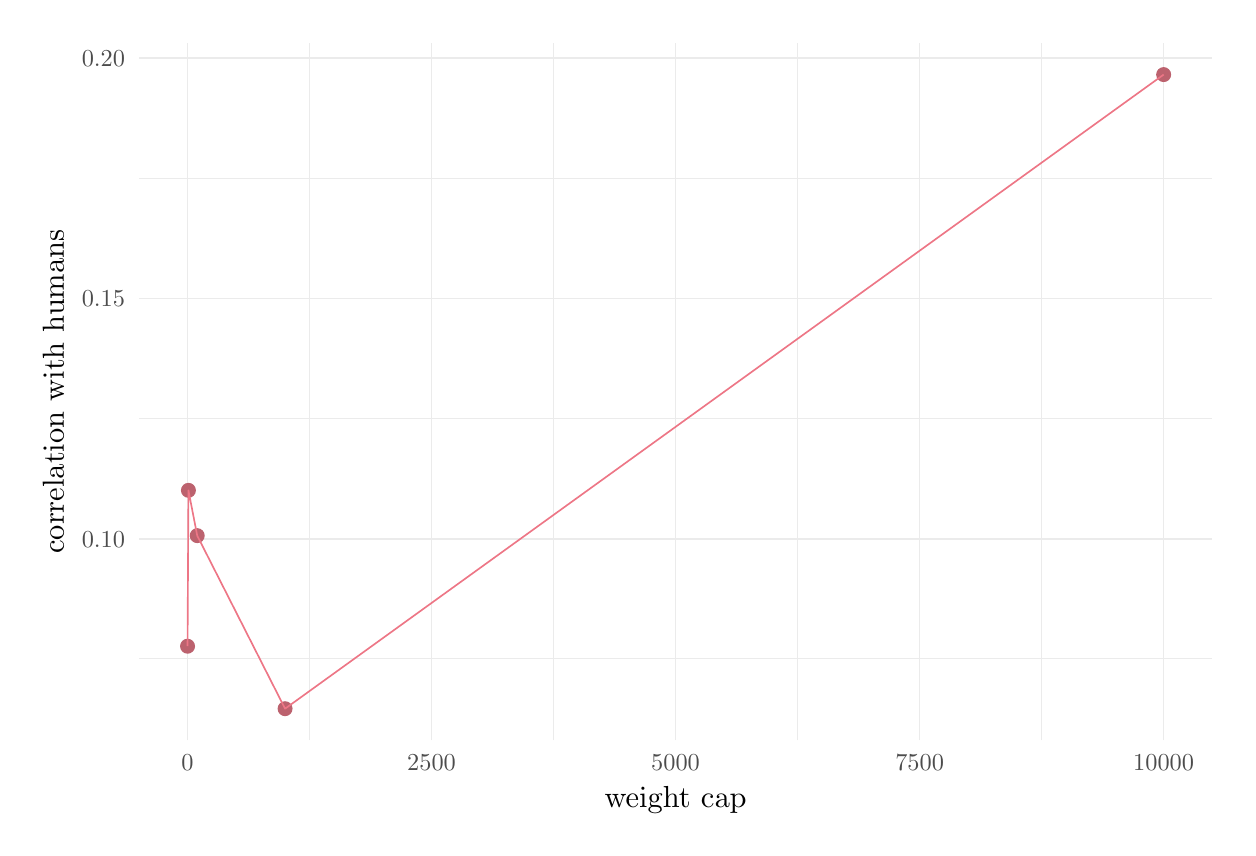
\begin{tikzpicture}[x=1pt,y=1pt]
\definecolor{fillColor}{RGB}{255,255,255}
\path[use as bounding box,fill=fillColor,fill opacity=0.00] (0,0) rectangle (433.62,289.08);
\begin{scope}
\path[clip] ( 40.14, 31.53) rectangle (428.12,283.58);
\definecolor{drawColor}{gray}{0.92}

\path[draw=drawColor,line width= 0.3pt,line join=round] ( 40.14, 60.99) --
	(428.12, 60.99);

\path[draw=drawColor,line width= 0.3pt,line join=round] ( 40.14,147.85) --
	(428.12,147.85);

\path[draw=drawColor,line width= 0.3pt,line join=round] ( 40.14,234.70) --
	(428.12,234.70);

\path[draw=drawColor,line width= 0.3pt,line join=round] (101.83, 31.53) --
	(101.83,283.58);

\path[draw=drawColor,line width= 0.3pt,line join=round] (190.02, 31.53) --
	(190.02,283.58);

\path[draw=drawColor,line width= 0.3pt,line join=round] (278.20, 31.53) --
	(278.20,283.58);

\path[draw=drawColor,line width= 0.3pt,line join=round] (366.39, 31.53) --
	(366.39,283.58);

\path[draw=drawColor,line width= 0.6pt,line join=round] ( 40.14,104.42) --
	(428.12,104.42);

\path[draw=drawColor,line width= 0.6pt,line join=round] ( 40.14,191.27) --
	(428.12,191.27);

\path[draw=drawColor,line width= 0.6pt,line join=round] ( 40.14,278.13) --
	(428.12,278.13);

\path[draw=drawColor,line width= 0.6pt,line join=round] ( 57.74, 31.53) --
	( 57.74,283.58);

\path[draw=drawColor,line width= 0.6pt,line join=round] (145.93, 31.53) --
	(145.93,283.58);

\path[draw=drawColor,line width= 0.6pt,line join=round] (234.11, 31.53) --
	(234.11,283.58);

\path[draw=drawColor,line width= 0.6pt,line join=round] (322.30, 31.53) --
	(322.30,283.58);

\path[draw=drawColor,line width= 0.6pt,line join=round] (410.48, 31.53) --
	(410.48,283.58);
\definecolor{drawColor}{RGB}{188,98,110}
\definecolor{fillColor}{RGB}{188,98,110}

\path[draw=drawColor,line width= 0.4pt,line join=round,line cap=round,fill=fillColor] ( 57.77, 65.57) circle (  2.50);

\path[draw=drawColor,line width= 0.4pt,line join=round,line cap=round,fill=fillColor] ( 58.09,121.89) circle (  2.50);

\path[draw=drawColor,line width= 0.4pt,line join=round,line cap=round,fill=fillColor] ( 61.27,105.52) circle (  2.50);

\path[draw=drawColor,line width= 0.4pt,line join=round,line cap=round,fill=fillColor] ( 93.01, 42.99) circle (  2.50);

\path[draw=drawColor,line width= 0.4pt,line join=round,line cap=round,fill=fillColor] (410.48,272.12) circle (  2.50);
\definecolor{drawColor}{RGB}{237,118,134}

\path[draw=drawColor,line width= 0.6pt,line join=round] ( 57.77, 65.57) --
	( 58.09,121.89) --
	( 61.27,105.52) --
	( 93.01, 42.99) --
	(410.48,272.12);
\end{scope}
\begin{scope}
\path[clip] (  0.00,  0.00) rectangle (433.62,289.08);
\definecolor{drawColor}{gray}{0.30}

\node[text=drawColor,anchor=base east,inner sep=0pt, outer sep=0pt, scale=  0.88] at ( 35.19,101.39) {0.10};

\node[text=drawColor,anchor=base east,inner sep=0pt, outer sep=0pt, scale=  0.88] at ( 35.19,188.24) {0.15};

\node[text=drawColor,anchor=base east,inner sep=0pt, outer sep=0pt, scale=  0.88] at ( 35.19,275.10) {0.20};
\end{scope}
\begin{scope}
\path[clip] (  0.00,  0.00) rectangle (433.62,289.08);
\definecolor{drawColor}{gray}{0.30}

\node[text=drawColor,anchor=base,inner sep=0pt, outer sep=0pt, scale=  0.88] at ( 57.74, 20.52) {0};

\node[text=drawColor,anchor=base,inner sep=0pt, outer sep=0pt, scale=  0.88] at (145.93, 20.52) {2500};

\node[text=drawColor,anchor=base,inner sep=0pt, outer sep=0pt, scale=  0.88] at (234.11, 20.52) {5000};

\node[text=drawColor,anchor=base,inner sep=0pt, outer sep=0pt, scale=  0.88] at (322.30, 20.52) {7500};

\node[text=drawColor,anchor=base,inner sep=0pt, outer sep=0pt, scale=  0.88] at (410.48, 20.52) {10000};
\end{scope}
\begin{scope}
\path[clip] (  0.00,  0.00) rectangle (433.62,289.08);
\definecolor{drawColor}{RGB}{0,0,0}

\node[text=drawColor,anchor=base,inner sep=0pt, outer sep=0pt, scale=  1.10] at (234.13,  7.44) {weight cap};
\end{scope}
\begin{scope}
\path[clip] (  0.00,  0.00) rectangle (433.62,289.08);
\definecolor{drawColor}{RGB}{0,0,0}

\node[text=drawColor,rotate= 90.00,anchor=base,inner sep=0pt, outer sep=0pt, scale=  1.10] at ( 13.08,157.56) {correlation with humans};
\end{scope}
\end{tikzpicture}


%}}
%
%\caption{\subref{sfig:scaling_f} Effect of scaling factor for facetted embeddings on the correlation on wordsim353. \subref{sfig:weight_cap} Effect of weight cap for facetted embeddings on the correlation on wordsim353.}
%\label{fig:correlation_change}
%\end{figure}
%
%
%\begin{figure}
%\centering
%\subcaptionbox{\label{sfig:full_men}}{
%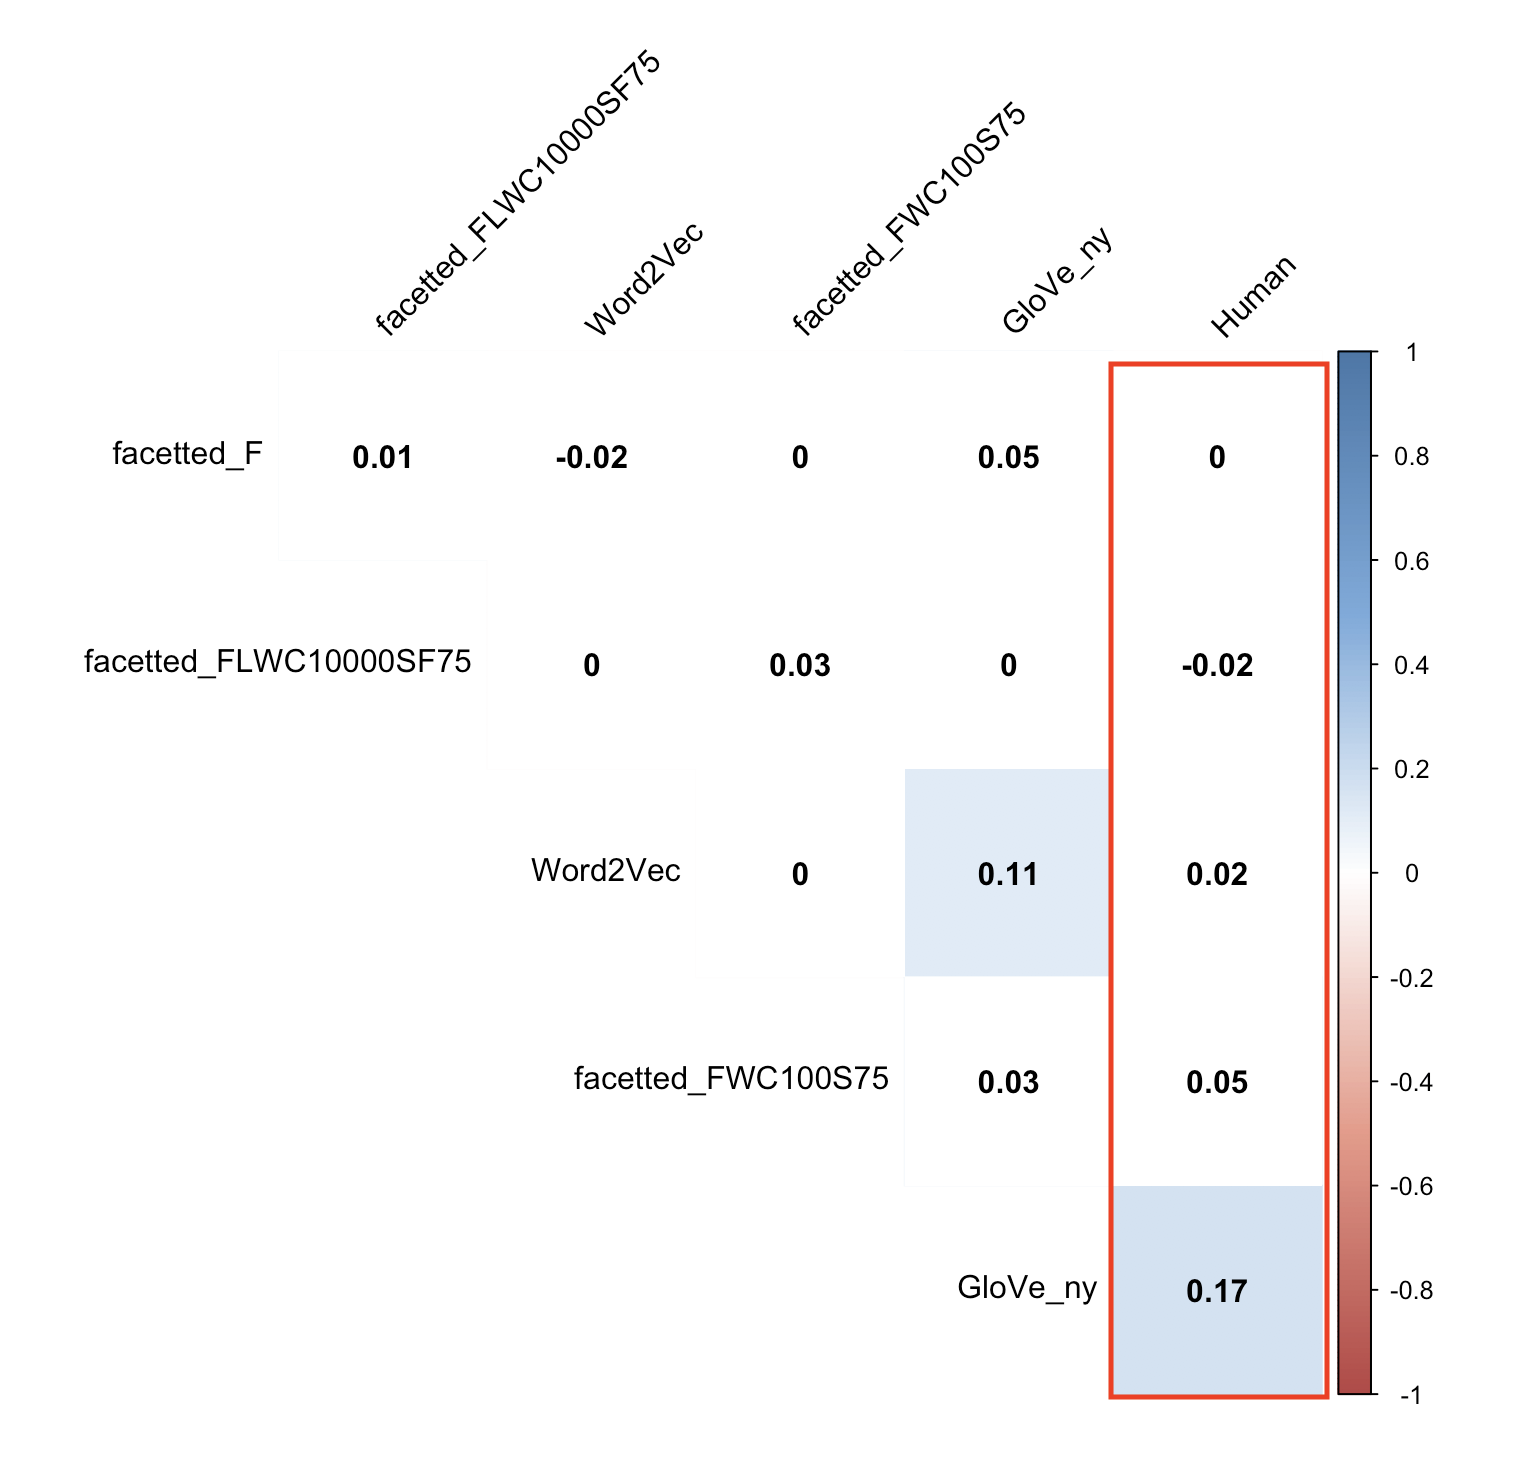
\includegraphics[width=0.7\linewidth , height=0.6\linewidth]{images/men_full.pdf}}
%\subcaptionbox{\label{sfig:part_men}}{
%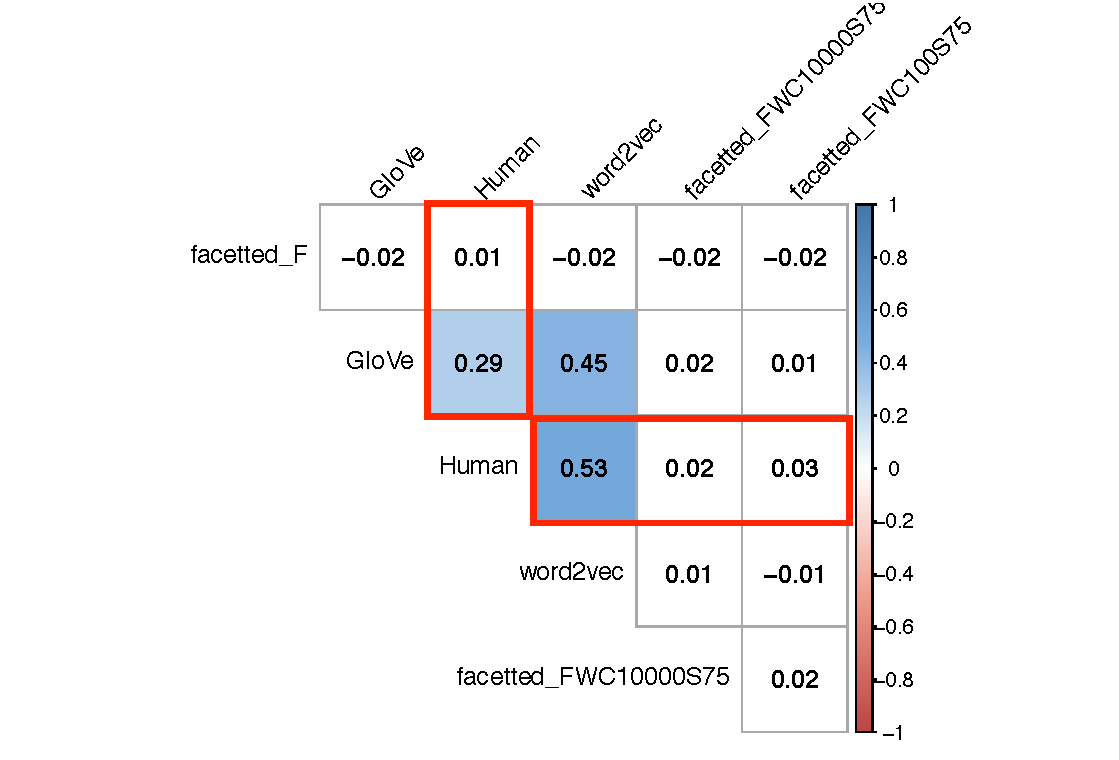
\includegraphics[width=0.7\linewidth , height=0.6\linewidth]{images/men_part.pdf}}
%
%\caption{Correlation plot of the relatedness scores on MEN using the~\subref{sfig:full_men} full vectors and ~\subref{sfig:part_men} using type-specific vectors. Red highlights show the correlation with the human annotations.}
%\label{fig:men_cor}
%\end{figure}
